%%%%%%%%%%%%%%%%%%%%%%%%%%%%%%%%%%%%%%%%%%%%%%%%%%
% Basic setup. Most papers should leave these options alone.
\documentclass[fleqn,usenatbib]{mnras}

% MNRAS is set in Times font. If you don't have this installed (most LaTeX
% installations will be fine) or prefer the old Computer Modern fonts, comment
% out the following line
\usepackage{newtxtext,newtxmath}
\usepackage{arydshln}
% Depending on your LaTeX fonts installation, you might get better results with one of these:
%\usepackage{mathptmx}
%\usepackage{txfonts}

% Use vector fonts, so it zooms properly in on-screen viewing software
% Don't change these lines unless you know what you are doing
\usepackage[T1]{fontenc}

% Allow "Thomas van Noord" and "Simon de Laguarde" and alike to be sorted by "N" and "L" etc. in the bibliography.
% Write the name in the bibliography as "\VAN{Noord}{Van}{van} Noord, Thomas"
\DeclareRobustCommand{\VAN}[3]{#2}
\let\VANthebibliography\thebibliography
\def\thebibliography{\DeclareRobustCommand{\VAN}[3]{##3}\VANthebibliography}

%%%%% AUTHORS - PLACE YOUR OWN PACKAGES HERE %%%%%
\usepackage{graphicx}	% Including figure files
\usepackage{amsmath,bm}	% Advanced maths commands
% \usepackage{amssymb}	% Extra maths sym
\usepackage[dvipsnames]{xcolor}
\usepackage{hyperref}
\usepackage{newtxtext,newtxmath}
\usepackage[T1]{fontenc}
\usepackage{adjustbox}
\usepackage{upgreek}
\usepackage{ulem,cancel}%for editing, to be removed before submission
\usepackage{nicefrac,xfrac}
\usepackage{academicons}
%%%%%%%%%%%%%%%%%%%%%%%%%%%%%%%%%%%%%%%%%%%%%%%%%%

%%%%% AUTHORS - PLACE YOUR OWN COMMANDS HERE %%%%%
%\newcommand{\RVOASA}{{\tt{R5}$\Omega$\tt{25S1}}}
%\newcommand{\RSOBSA}{{\tt{R5}$\Omega$\tt{60S1}}}
%% \newcommand{\RSclem}{{\tt{R5}$\Omega$\tt{clem}}}
%\newcommand{\RSclem}{{\tt{R5}$\Omega$\tt{MW}}}
%\newcommand{\RSOBSB}{{\tt{R5}$\Omega$\tt{60S07}}}
%\newcommand{\RSOBSC}{{\tt{R5}$\Omega$\tt{60S05}}}
%\newcommand{\RSOBSD}{{\tt{R5}$\Omega$\tt{60S03}}}
%\newcommand{\CM}{{\tt{R5}$\Omega$\tt{60S03CM}}}
%\newcommand{\RSOBSE}{{\tt{R5}$\Omega$\tt{60S01}}}
%\newcommand{\RXOASA}{{\tt{R10}$\Omega$\tt{25S1}}}
%\newcommand{\RAOASA}{{\tt{R05}$\Omega$\tt{25S1}}}
%\newcommand{\RAOASACM}{{\tt{R05}$\Omega$\tt{25S1CM}}}
%\newcommand{\RBOASACM}{{\tt{R17}$\Omega$\tt{50S1CM}}}
\newcommand{\RVOASA}{{\sf{O25}}}
\newcommand{\RSOBSA}{{\sf{O60}}}
% \newcommand{\RSclem}{{\tt{R5}$\Omega$\tt{clem}}}
\newcommand{\RSclem}{{\sf{OMW}}}
\newcommand{\RSOBSB}{{\sf{O60q0.7}}}
\newcommand{\RSOBSC}{{\sf{O60q0.5}}}
\newcommand{\RSOBSD}{{\sf{O60q0.3}}}
\newcommand{\CM}{{\sf{O60q0.3cr}}}
\newcommand{\RSOBSE}{{\sf{O60q0.1}}}
\newcommand{\RXOASA}{{\sf{H25}}}
\newcommand{\RAOASA}{{\sf{G25}}}
\newcommand{\RAOASACM}{{\sf{G25cr}}}
\newcommand{\RBOASACM}{{\sf{G50cr}}}

\definecolor{midblue}{rgb}{0.0,0.4,0.7}
\definecolor{mypurple}{rgb}{0.7,0.3,0.8}

\definecolor{PineGreen}{HTML}{008B72}
\definecolor{Berry}{HTML}{FF2052}
\newcommand{\fg}[1]{\textcolor{cyan}{#1}} %Edited text to be visible to others
\newcommand{\fgs}[1]{\textcolor{cyan}{\sout{#1}}}
\newcommand{\fag}[1]{\textcolor{cyan}{[FAG: #1]}} %Comment in the text to other authors
\newcommand{\yq}[1]{\textcolor{PineGreen}{#1}} %Edited text to be visible to others
\newcommand{\Yq}[1]{\textcolor{PineGreen}{[YQ: #1]}} %Comment in the text to other authors
\newcommand{\as}[1]{\textcolor{mypurple}{#1}} %Edited text to be visible to others
\newcommand{\ass}[1]{\textcolor{mypurple}{\sout{#1}}}
\newcommand{\AS}[1]{\textcolor{red}{[AS: #1]}} %Comment in the text to other authors
\newcommand{\dvt}[1]{\textcolor{Berry}{#1}} %Edited text to be visible to others
\newcommand{\Devika}[1]{\textcolor{Berry}{[DT: #1]}} %Comment in the text to other authors
\newcommand{\AB}[1]{\textcolor{SpringGreen}{#1]}} %Comment in the text to other authors

\newcommand{\gafd}{Geophys.\ Astrophys.\ Fluid Dyn.}
\newcommand{\jfm}{J.~Fluid. Mech.}

\newcommand\aver[1]{\langle#1\rangle}%partial derivative

\newcommand{\dd}{\mathrm{d}}        %differential
\newcommand\e{\mathrm{e}} %Euler's constant
\newcommand\ii{\mathrm{i}} %imaginary unity
\newcommand\sound{_\text{s}} %subscript sound
\newcommand\D{_\text{D}} %subscript dynamo
\newcommand\deriv[2]{\frac{\partial#1}{\partial#2}}%partial derivative
\newcommand\oderiv[2]{\frac{\od#1}{\od#2}}%ordinary derivative
\newcommand\dderiv[2]{\frac{\text{D}#1}{\text{D}#2}}%Lagrangian derivative
%\newcommand\mean[1]{\overline{#1}}% average
\newcommand\mean[1]{\langle #1\rangle}% ensemble average
\newcommand\meanh[1]{{\langle #1\rangle}_{xy}}% horizontal average
\renewcommand\vec[1]{\bm{#1}}% vector convention
%\renewcommand{\vec}[1]{{{\boldmath #1}}}%also makes bold Greek letters
\newcommand\kin{_\text{k}} %subscript kinetic
\newcommand\magn{_\text{m}} %subscript magnetic
\newcommand{\BB}{\vec{B}} %Bold B
\newcommand{\mB}{\langle\vec{B}\rangle} %Bold B
\newcommand{\bb}{\vec{B}^\prime} %Bold b
\newcommand{\U}{\vec{u}} %Bold U
\newcommand{\mU}{\langle\vec{u}\rangle} %Bold B
\newcommand{\uu}{\vec{u}^\prime} %Bold b
\renewcommand{\mathbfss}[1]{{{\mbox{\boldmath{$#1$}}}}}

\DeclareMathAlphabet{\mathsc}{OT1}{cmr}{m}{sc}
\def\testbx{bx}%
\DeclareRobustCommand{\ion}[2]{%
\relax\ifmmode
\ifx\testbx\f@series
{\mathbf{#1\,\mathsc{#2}}}\else
{\mathrm{#1\,\mathsc{#2}}}\fi
\else\textup{#1\,{\mdseries\textsc{#2}}}%
\fi}

\DeclareMathOperator{\sign}{sign}
% Please keep new commands to a minimum, and use \newcommand not \def to avoid
% overwriting existing commands. Example:
%\newcommand{\pcm}{\,cm$^{-2}$}	% per cm-squared

%UNITS#####################################################
%       distance ------------------------------------------
\newcommand{\A}{\,text{\AA}} %Angstrom
\newcommand{\AU}{\,{\rm AU}} %Astronomical unit
\newcommand{\mkm}{\,\mu{\rm m}} %micro metre
\newcommand{\mm}{\,{\rm mm}}    %mm
\newcommand{\cm}{\,{\rm cm}}    %cm
\newcommand{\km}{\,{\rm km}}    %km
\newcommand{\m}{\,{\rm m}}      %m
\newcommand{\Mm}{\,{\rm Mm}}    %Megametre
%
\newcommand{\p}{\,{\rm pc}}     %parsec
\newcommand{\kpc}{\,{\rm kpc}}  %kpc
\newcommand{\Mpc}{\,{\rm Mpc}}  %Mpc
% mass/amount of matter ------------------------------
\newcommand{\g}{\,{\rm g}}      %gramm
\newcommand{\kg}{\,{\rm kg}}    %kg
\newcommand{\mol}{\,{\rm mol}}  %mole
% time/frequency -------------------------------------
\newcommand{\days}{\,{\rm d}}   %days
\newcommand{\GHz}{\,{\rm GHz}}  %GHz
\newcommand{\Hz}{\,{\rm Hz}}    %Hz
\newcommand{\kHz}{\,{\rm kHz}}  %kHz
\newcommand{\MHz}{\, {\rm MHz}} %MHz
\newcommand{\nHz}{\,{\rm nHz}}  %nHz
\newcommand{\s}{\,{\rm s}}      %seconds
%
\newcommand{\yr}{\,{\rm yr}}    %years
\newcommand{\Myr}{\,{\rm Myr}} %Megayears
\newcommand{\Gyr}{\,{\rm Gyr}}  %Gigayears
% speed ------------------------------------------
\newcommand{\cms}{\cm\s^{-1}}    %cm/s
\newcommand{\kms}{\km\s^{-1}}    %km/s
% electric & magnetic fields ------------------------------------------
\newcommand{\G}{\,{\rm G}}      %Gauss
\newcommand{\kG}{\,{\rm kG}} %kiloGauss
\newcommand{\mG}{\,{\rm mG}}    %MegaGauss
\newcommand{\mkG}{\,\upmu{\rm G}} %microGauss
\newcommand{\nG}{\,{\rm nG}} %nanoGauss
\newcommand{\Mx}{\,{\rm Mx}}    %Maxwell
\newcommand{\V}{\,{\rm V}} %%Volt
\newcommand{\kV}{\,{\rm kV}}    %kiloVolt
\newcommand{\T}{\,{\rm T}} %%Tesla
% temperature/force/energy/radiation flux ------------------------------
\newcommand{\C}{\,{\rm ^\circ C}}      %Celsius
\newcommand{\dyn}{\,{\rm dyn}}  %dyne
\newcommand{\erg}{\,{\rm erg}}  %erg
\newcommand{\eV}{\,{\rm eV}}  %electronvolt
\newcommand{\keV}{\,{\rm keV}}  %kilo electron volt
\newcommand{\MeV}{\,{\rm MeV}}  %mega electron volt
\newcommand{\GeV}{\,{\rm GeV}}  %giga electron volt
\newcommand{\TeV}{\,{\rm TeV}}  %tera electron volt
\newcommand{\K}{\,{\rm K}}      %Kelvin
\newcommand{\Jo}{\,{\rm J}}      %Joule
\newcommand{\Jy}{\,{\rm Jy}}    %Jansky
\newcommand{\Jyb}{\,{\rm Jy/beam}} %Jansky per beam
\newcommand{\mJy}{\,{\rm mJy}}          %milliJansky
\newcommand{\mJyb}{\,{\rm mJy/beam}}    %milliJansky per beam
\newcommand{\mkJy}{\,\mu{\rm Jy}}          %milliJansky
\newcommand{\mkJyb}{\,\mu{\rm mJy/beam}}    %milliJansky per beam
\newcommand{\kW}{\,{\rm kW}}    %kiloWatt
\newcommand{\MW}{\,{\rm MW}}    %MegaWatt (for writing about power stations)
\newcommand{\W}{\,{\rm W}} %Watt

%%%%%%%%%%%%%%%%%%%%%%%%%%%%%%%%%%%%%%%%%%%%%%%%%%

%%%%%%%%%%%%%%%%%%% TITLE PAGE %%%%%%%%%%%%%%%%%%%

% Title of the paper, and the short title which is used in the headers.
% Keep the title short and informative.
\title[Non-linear magnetic buoyancy and galactic dynamos]{Non-linear magnetic buoyancy instability and galactic dynamos}

% The list of authors, and the short list which is used in the headers.
% If you need two or more lines of authors, add an extra line using \newauthor
\author[Y.~Qazi et al.]{Yasin Qazi,$^{1}$\thanks{E-mails: Y.Qazi@newcastle.ac.uk (YQ), anvar.shukurov@ncl.ac.uk (AS), devika.tharakkal@helsinki.fi (DT), frederick.gent@aalto.fi (FAG), abhijit.bendre@epfl.ch (ABB)}\href{https://orcid.org/0009-0008-9513-8761}{
\includegraphics[scale=0.5]{orcid_16x16.jpeg}}
A.~Shukurov,$^{1}$\href{https://orcid.org/0000-0001-6200-4304}{
\includegraphics[scale=0.5]{orcid_16x16.jpeg}}
D.~Tharakkal,$^{1,2}$\href{https://orcid.org/0000-0002-4563-2277}{
\includegraphics[scale=0.5]{orcid_16x16.jpeg}}
F.~A.~Gent$^{3,4,1}$\href{https://orcid.org/0000-0002-1331-2260}{
\includegraphics[scale=0.5]{orcid_16x16.jpeg}}
\&
A.~B.~Bendre$^{5}$\href{https://orcid.org/0000-0001-5208-8989}{
\includegraphics[scale=0.5]{orcid_16x16.jpeg}}
\\
% List of institutions
$^{1}$School of Mathematics, Statistics and Physics, Newcastle University, Newcastle upon Tyne, NE1 7RU, UK\\
$^{2}$Department of Physics, University of Helsinki, PO Box 64, FI-00014, Helsinki, Finland\\
$^{3}$Astroinformatics, Department of Computer Science, Aalto University, PO Box 15400, FI-00076, Espoo, Finland\\
$^{4}$Nordita, KTH Royal Institute of Technology and Stockholm University, Hannes Alfv\'ens v\"ag 12, Stockholm, SE-106, Sweden\\
$^{5}$Scuola Normale Superiori di Pisa, P.za dei Cavalieri, 7, 56126 Pisa, Italy
}

% These dates will be filled out by the publisher
\date{Accepted XXX. Received YYY; in original form ZZZ}

% Enter the current year, for the copyright statements etc.
\pubyear{2024}

% Don't change these lines
\begin{document}
\label{firstpage}
\pagerange{\pageref{firstpage}--\pageref{lastpage}}
\maketitle

% Abstract of the paper
\begin{abstract}
The magnetic buoyancy and Parker instabilities are strong and generic
instabilities expected to occur in most astrophysical systems with sufficiently
strong magnetic fields.  In galactic and accretion discs, large-scale magnetic
fields are thought to result from the mean-field dynamo action, in particular,
the $\alpha^2\Omega$-dynamo. Using non-ideal MHD equations, we model a section
of the galactic disc in which the large-scale magnetic field is generated by an
imposed $\alpha$-effect and differential rotation. We extend our earlier study
of the interplay between magnetic buoyancy and the mean-field dynamo. We add
differential rotation which enhances the dynamo and cosmic rays which enhance
magnetic buoyancy.  We construct a simple 1D model which replicates all
significant features of the 3D simulations.  We confirm that magnetic buoyancy
can lead to oscillatory magnetic fields and discover that it can {vary} the
magnetic field parity between quadrupolar and dipolar{,} and that inclusion
of the differential rotation is responsible for the switch in field parity.
Our results suggest that the large-scale magnetic field can have a dipolar
parity within a few kiloparsecs of the galactic centre, while quadrupolar
parity can remain predominant in the outer parts of a galactic disc.  Cosmic
rays with magnetic buoyancy dominant supports oscillatory nonlinear states, a
spatial magnetic field structure similar to the alternating magnetic field
directions observed in some edge-on galaxies.
\end{abstract}

% Select between one and six entries from the list of approved keywords.
% Don't make up new ones.
\begin{keywords}
instabilities -- magnetic fields -- MHD -- dynamo -- galaxies: magnetic fields -- ISM: structure
\end{keywords}

%%%%%%%%%%%%%%%%% BODY OF PAPER %%%%%%%%%%%%%%%%%%

\section{Introduction}

The magnetic buoyancy instability (MBI) \citep{N61}, or the magnetic
Rayleigh-Taylor instability is a fundamental process that affects magnetic
fields in stratified plasmas. It develops wherever the strength of a magnetic
field decreases sufficiently rapidly against the gravitational acceleration.
Typical situations where this can arise are in the thin magnetised plasma layer
of galactic \citep{Rodrigues2016,KNPS19,SBADMN19} and accretion discs
\citep{VB97,BH98,Blackman12,JSD14}.  Under the hydrostatic equilibrium, both
magnetic field strength and gas density usually decrease with distance $z$ from
the midplane layer. Since the magnetic field has pressure but not weight, the
gas density is reduced near the midplane where the magnetic field is stronger,
producing an unstable structure.

The interstellar medium of spiral galaxies also contains cosmic rays which have
negligible weight but exert a dynamically significant pressure. The MBI
enhanced by cosmic rays is known as the Parker instability \citep{Parker1979}.
This ubiquitous instability has a time scale (of the order of the sound or
Alfv\'en crossing time based on the density scale height) much shorter than the
lifetimes of the astrophysical objects, and it must be in its nonlinear state
in virtually any object prone to it. The linear stages of both instabilities
are well understood and their dispersion relations have been obtained for a
variety of physical models \citep[e.g.,][see also \citealt{SS21} and references
therein]{Giz1993,FT94,FT95,Kim1997,Rodrigues2016,DT2022a}.

The nonlinear, quasi-stationary states of the MBI and Parker instability are
much less understood, in particular, because they require numerical
simulations.  \citet{DT2022a,DT2022b} investigated them in the case of an
imposed planar, unidirectional magnetic field. In a non-rotating system, the
instability leads to a state with large scale heights of both magnetic field
and cosmic rays, the gas layer is correspondingly thin as it is supported
solely by the thermal pressure gradient (and turbulent pressure if available)
\citep{DT2022a}.

Rotation changes the nonlinear state significantly because gas motions driven
by the instability become helical and can act as a mean-field dynamo
\citep[e.g.,][see also \citealt{HL1997a} and \citealt{1999MOSS} and references
therein]{DT2022b}. As a result, even in the presence of imposed magnetic field,
the magnetic field near the midplane changes profoundly and can reverse its
direction in what appears to be a nonlinear, long-period oscillation. Similar
magnetic field reversals occur in the simulations of \citet{JoLe08},
\citet{GJL12} and \citet{MNKASM2013}.

Large-scale magnetic fields in galaxies and accretion discs are produced by a
mean-field ($\alpha$-effect) dynamo \citep[][and references therein]{SS21}, and
\cite{QSTGB23} explore the nonlinear instability of a the magnetic field
generated by the imposed $\alpha$-effect rather than introduced directly via
initial, boundary or background conditions. Rotation is neglected in this model
to simplify the interaction of the dynamo and the MBI. Magnetic fields
generated by the $\alpha$-effect are helical, and the Lorentz force drives
helical motions which act as a dynamo even without any explicit rotation. As a
result, the system develops nonlinear oscillations similar in their origin to
those observed by \citet{DT2022b} in a rotating system with an imposed
non-helical magnetic field.

Here we extend the model of \citet{QSTGB23} to explore the effects of rotation
and cosmic rays on the MBI. We show that the response of the dynamo action to
the instability is even more profound, and the large-scale magnetic field not
only becomes oscillatory, but it can change its parity from quadrupolar (where
the horizontal magnetic field is symmetric with respect to the midplane) to
dipolar state (where the horizontal field is antisymmetric). In this paper, we
seek to reveal, verify and understand these unexpected features of the
nonlinear MBI and Parker instability.  Our results are reproduced by a modified
version of the {1D} model introduced by \citet{QSTGB23}. Despite its
simplicity, the model is so successful that it has its own value in exploring
nonlinear instability.

Apart from a model for the Solar vicinity of the Galaxy, we present simulations
of a galaxy with parameters typical of the inner parts of spiral galaxies. Our
results are consistent with the complicated structure of the global galactic
magnetic fields with large-scale direction reversals as revealed by
observations of the Faraday rotation \citep[see section~3.4.3 of][for a
review]{IB+24}. We are not aware of other convincing explanations of such
complex magnetic structures in galaxies.

Our results show that a quadrupolar magnetic field produced by the mean-field
dynamo action in a thin disc \citep{SS21} can be transformed into a dipolar
field by the magnetic buoyancy in a rapidly rotating system. This gives
credence to the claims that the global magnetic field within a few kiloparsecs
from the centre of the Milky Way has the dipolar parity \citep{Han17}.

The numerical model used is explained in Section~\ref{sec:Equations}.  Our
simulation results are reported in Section~\ref{sec:Results} in which we
discuss the evolution of the dynamo and MBI in our solutions in
Section~\ref{sec:Rotation} the effects of model parameters on the growth rates
in Section~\ref{sec:params} on  the parity of the magnetic field in
Section~\ref{sec:parity}. The effects of cosmic rays are included in
Section~\ref{sec:CM}.  We also consider viscosity and magnetic diffusivity
similar in magnitude to those produced by the supernova-driven turbulence in
spiral galaxies. In Section~\ref{sec:interp} we seek to interpret the
results{, examining the $\alpha$-effect during the each stage of the dyanmo
and MBI, Section~\ref{sec:approx}, turbulent transprot coefficient composition
of} the electromotive force (EMF) in Section~\ref{sec:emf} {and to verify}
our interpretation of the results in Section~\ref{sec:1D} {we enhance} the
one-dimensional model introduced in Section~$4.1$ of \citet{QSTGB23}.
Section~\ref{sec:Summary} summarizes our results {and conclusions}.

%-----------------------------------------
\section{Model description}\label{sec:Equations}

The model and simulations used here are very similar to those of
\citet{QSTGB23} but now include differential rotation. We model isothermal gas
and magnetic field within a {three-dimensional (3D)} Cartesian box with
$x,y$ and $z$ representing the radial, azimuthal and vertical directions,
respectively. The simulation domain extends $4\kpc$ in each horizontal
direction and $3\kpc$ vertically, centred at the galactic midplane. We have
tested computational boxes of various sizes from $0.5\kpc$ to $16\kpc$ to
confirm that we capture all essential features of the system. The grid
resolution is $256\times256\times192$ mesh points with a grid spacing of about
$15.6 \p$ along each dimension. The domain size is larger than the expected
vertical and horizontal scales of the instability, and the resolution is
sufficient to obtain convergent solutions.

Table~\ref{tab:parameter_values} summarizes the {common} parameter values
adopted in this study, while Table~\ref{tab:sims} {lists the parameters used
and some indicative results obtained for each simulation} discussed in this
paper.
%---------------------------------------------------------------------
\subsection{Basic equations}

We solve a system of isothermal non-ideal compressible MHD equations using the
sixth-order in space and third-order in time finite-difference \textsc{Pencil
Code} \citep{brandenburg2002,Pencil-JOSS}.  In the local rotating Cartesian
frame $(x,y,z)$, the governing equations are
%------------------------------------------------------------------------
\begin{align}
    \dderiv{\rho}{t} &= -\rho\nabla \cdot \U +\nabla \cdot(\zeta_D\nabla\rho)\,,
            \label{eq:mass_conservation}\\
    \dderiv{\U}{t} &= -g\hat{\vec{z}} - \frac{\nabla P}{\rho}
        +\frac{(\nabla\times\BB)\times\BB}{4\pi\rho}
        +\frac{\nabla\cdot(2\rho\nu{\mathbfss{\uptau}})}{\rho}
        -Su_x\vec{\hat{y}}
        -2\vec{\Omega}\times \mathbf{u}        \nonumber\\
    \label{eq:momentum}
        &\mbox{}\quad +\nabla\left(\zeta_{\nu}\nabla \cdot \U \right)
        +\nabla\cdot \left(2\rho\nu_6{\mathbfss{\uptau}}^{(5)}\right)
        -\dfrac{1}{\rho}\U\nabla\cdot\left(\zeta_D\nabla\rho\right)\,,\\
    \deriv{\vec{A}}{t} &=  \alpha \BB+ \U\times \BB - SA_y\vec{\hat{{x}}} - Sx\frac{\partial \mathbf{A}}{\partial y} -\eta \nabla\times \BB
    \label{eq:induction}
    +\eta_6\nabla^{(6)}\vec{A}\,,
\end{align}
%-------------------------------------------------------------------
for the gas density $\rho$, the velocity $\vec{u}$ of the deviations from the
overall rotational pattern and the magnetic vector potential $\vec{A}$. The
vertical gravitational acceleration is $g$, the thermal pressure $P$, the
magnetic field $\BB=\nabla\times\vec{A}$  and the local angular velocity
$\vec{\Omega}=(0,0,\Omega)$. The physical viscosity and magnetic diffusivity
are $\nu$ and $\eta$, respectively, and $\alpha$ (see
Section~\ref{sect:modelmf}) contributes the $\alpha$-effect that maintains a
large-scale magnetic field via the mean-field dynamo action. The latter is
introduced because we do not include turbulent motions driven by supernovae
which are responsible for the $\alpha$-effect. We note, however, that the
motions driven by the instability also become helical under the action of the
large-scale shear, and this is fully captured by these simulations.

%------------------------------------------------------------------------
\begin{table}
\caption{
Parameters common to all models applying the % adopted in the numerical
solutions of
equations~\eqref{eq:mass_conservation}--\eqref{eq:induction} to %. in
Sections~\ref{sec:Rotation}--\ref{sec:1D}.
\label{tab:parameter_values}
}
\centering
\begin{tabular}{llll}
\hline
Quantity                   & Symbol          & Value           &Unit     \\
\hline
Grid spacing            & $\updelta\vec{x}$  & 0.0156          &kpc \\
Sound speed                 & $c\sound$          & 15          &km$\s^{-1}$ \\
Initial gas column density  &$\Sigma$            & $10^{21}$   & cm$^{-2}$\\
Shock-capturing viscosity   & $\nu_\text{shock}$ & 1           & kpc$^{2}$\\
Shock-capturing diffusivity & $D_\text{shock}$   & 1           & kpc$^{2}$\\
Hyper-diffusivities & $\nu_6,\ \eta_6$  & $10^{-12}$ &kpc$^{5}\kms$\\
\hline
\end{tabular}
\end{table}
%------------------------------------------------------------------------

%------------------------------------------------------------------------
\begin{table*}
    \centering
    \caption{MHD simulation model parameters, characteristics and summary
results. Magnitude of the $\alpha$-effect is $\alpha_0$, turbulent magnetic
diffusivity is $\eta$ and dynamo scale height is $h_\alpha$. Galactic rotation
and rate of shear are $\Omega$ and $S$, respectively, with $S=R\,\dd\Omega/\dd
R$, in which $R$ is the galactocentric radius.  {The ratio $q=-S/\Omega=1$,
unless otherwise stated.} From these model parameters, we derive the dynamo
characteristic numbers $R_{\alpha}$ and $R_{\omega}$, given in \eqref{Ral},
which quantify the large-scale magnetic induction effects and dynamo action due
to the $\alpha$-effect and differential rotation, respectively, which determine
the dynamo number $D$.  Summary result $\gamma\D$ is the rate of the
exponential growth of the magnetic field strength during the linear phase of
the dynamo and $\gamma_{u}$ is the corresponding growth rate of the
root-mean-square gas speed, due to the subsequent onset of MBI. The parity
indicates the dominant qualitative effect on the magnetic field of the MBI. The
first two models have turbulent viscosity $\nu=0.008\kpc\kms$ models in
\citet{QSTGB23}, otherwise $\nu=0.3\kpc\kms$.  {Model \RXOASA\ has the
highest $R_\alpha=10$, while models with $R_\alpha=5$ are denoted by {\sf{O}},
models relevant to observed galactic parameters are denoted by {\sf{G}} and
subscript {\sf{cr}} indicates cosmic rays are included.}}
%The last three models adopt realistic parameters taken from disk glalaxies. CM appended to the model name indicates cosmic rays are included.}
\begin{tabular}{l|ccccc|ccc|ccc}
\cline{1-12}
 Model    &$\alpha_0$  &$\eta$               &$h_\alpha$&$\Omega$                   &$S$                        &$R_\alpha$&$R_\omega$&$D$  &$\gamma\D$  &$\gamma_u$   &   Magnetic     \\
          &\![$\kms$]\!&\![km$\s^{-1}\kpc$]\!&[pc]      &\!$[\!\kms\!\kpc^{-1}\!]$\!&\!$[\!\kms\!\kpc^{-1}\!]$\!&          &          &      &[Gyr$^{-1}$]& [Gyr$^{-1}$]&   parity  \\
\cline{1-12}
 \RVOASA  &0.75        & 0.03                &200       &25                         &   $-25$                   &    5     &   $-33.4$&-167  & 1.5        &   10.5      &    Dipolar     \\
 \RXOASA  &1.5         & 0.03                &200       &25                         &   $-25$                   &    10    &   $-33.4$&-334  & 14.1       &          &    Quadrupolar \\
 \RSOBSA  &5           & 0.3                 &300       &60                         &   $-60$                   &    5     &   $-18.0$& -90  & 6.1        &   12.4      &    Quadrupolar \\
 \RSOBSB  &5           & 0.3                 &300       &60                         &   $-42$                   &    5     &   $-12.6$& -63  & 13.3       &   26.7      &    Dipolar     \\
 \RSOBSC  &5           & 0.3                 &300       &60                         &   $-30$                   &    5     &   $-9.0$ & -45  & 16.4       &   32.5      &    Dipolar     \\
 \RSOBSD  &5           & 0.3                 &300       &60                         &   $-18$                   &    5     &   $-5.4$ & -27  & 17.5       &   34.5      &    Dipolar     \\
 \RSOBSE  &5           & 0.3                 &300       &60                         &   $-9$                    &    5     &   $-1.8$ & -9   & 14.1       &   28.2      &    Dipolar     \\
 \CM      &5           & 0.3                 &300       &60                         &   $-9$                    &    5     &   $-1.8$ & -9   & 15.9       &   18.0      &    Dipolar     \\
 \RAOASA  &0.3         & 0.3                 &500       &25                         &   $-25$                   &    0.5   &   $-20.8$& -10.4& 1.2        &   1.0      &    Quadrupolar \\
 \RAOASACM&0.3         & 0.3                 &500       &25                         &   $-25$                   &    0.5   &   $-20.8$& -10.4& 1.4        &   1.6      &    Quadrupolar \\
 \RBOASACM&2.5         & 0.3                 &200       &50                         &   $-50$                   &    1.7   &   $-6.7$ & -11.4& 5.4        &   2.1       &    Quadrupolar \\
\cline{1-12}
\end{tabular}
    \label{tab:sims}
\end{table*}
%---------------------------------------------------------------------

The advective derivative is $\text{D}/\text{D}t= \partial/\partial t +
(\vec{U}+\vec{u})\cdot\nabla$ with $\vec{U} = (0,Sx,0)$ the global shear flow
(differential rotation) in the local Cartesian coordinates.  The shear rate is
$S$ (= $R\,\dd\Omega/\dd R$ in terms of the cylindrical radius $R$); for a flat
rotation curve, $\Omega \propto R^{-1}$ and $S = -\Omega$. We neglect the
vertical gradients of the $\Omega$ and $S$ since the observed magnitude of the
vertical gradient of $\vec{U}$ is of the order of $20 \kms \kpc^{-1}$ (section
10.2.3 of \citealt{SS21}, and references therein), leading to a relatively
small velocity lag of order $30\kms$ at $|z| = 1.5 \kpc$.

We use the gravitational acceleration obtained for the Solar neighbourhood of
the Milky Way by \citet{K&G1989MNRAS} (see Section~\ref{sect:modelmf}), scaled
appropriately when we consider inner parts of a galaxy. The isothermal gas has
the sound speed $c\sound = 15 \kms$, which corresponds to a temperature of $T
\approx 2\times 10^4\K$.

The traceless rate of strain tensor $\uptau$ has the form $\tau_{ij} =
\frac{1}{2}(\partial_j u_i + \partial_i u_j)$ (where, where $\partial_i$ =
$\partial/\partial x_{i}$ and summation over repeated indices is understood.).
Hyperdiffusion with constant coefficients $\nu_6$ and $\eta_6$ is used to
resolve grid-scale instabilities, with $\tau_{ij}^{(5)} = \frac{1}{2}\left[
\partial^5_i u_j + \partial^4_i(\partial_j u_i) \right] -
\frac{1}{6}\partial^4_i(\delta_{ij}\partial_k u_k)$ and $\nabla^{(6)} A_i =
\partial^3_j\partial^3_j A_i$, where $\partial_i^n = \partial^n/\partial x^n_i$
\citep{ABSG2002,Gent2021}.

The artificial viscosity to resolve shocks $\zeta_\nu = \nu_{\rm shock}f_{\rm
shock}$ in equation~\eqref{eq:momentum}, where $f_{\rm shock} \propto |\nabla
\cdot \vec{u}|_{-\rm ve}$ is non-zero only in convergent flows \citep[see,
e.g.,][]{Gent2020}.  Following \citet{Gent2020}, we also include the terms with
$\zeta_D=D_{\rm shock}f_{\rm shock}$ in equation~\eqref{eq:mass_conservation}
to ensure the momentum conservation in Equation~\eqref{eq:momentum}.

The initial conditions conform to a hydrostatic equilibrium aside from the
inclusion of a negligible random magnetic field.  The seed magnetic field
applied comprises Gaussian random noise in the vector potential component $A_z$
with a mean amplitude proportional to $\rho^{1/2}(z)$ and the maximum strength
$10^{-6}\mkG$ at $z=0$, such that $B_z=0$. A random initial magnetic field
leads to shorter transients than is the case for a unidirectional initial
field.

%---------------------------------------------------------------------
\subsection{Boundary conditions}

The boundary conditions in horizontal directions are periodic for all variables
in the $y$ (azimuthal) direction and sliding-periodic along $x$ (radius) to
allow for the differential rotation. To prevent an artificial inward advection
of the magnetic energy through the top and bottom of the domain at $z=\pm
1.5\kpc$, we impose there the conditions $B_x=B_y = \partial B_z/\partial z=0$.
The boundary conditions for the horizontal velocity are stress-free,
\begin{equation}
    \deriv{u_z}{z} = \deriv{u_y}{z} = 0,\quad \text{at } |z| = 1.5\,.
\end{equation}
To permit vertical gas flow across the boundaries without exciting numerical instabilities, the boundary condition for $u_z$ imposes the boundary outflow speed across the ghost zones outside the domain whereas an inflow speed at the boundary tends smoothly to zero across the ghost zones \citep{Gent_SN_ISM_1}. The density gradient is kept at a constant level at the boundaries, with the scale height intermediate between that of the Lockman layer and the galactic halo,
\begin{equation}
    \deriv{\ln\rho}{z} = \pm \frac{1}{0.9\kpc} \quad \text{at } z = \mp 1.5\kpc\,,
\end{equation}
and we note that the value of the scale height imposed at the boundaries has a negligible effect on the results.

%---------------------------------------------------------------------
\subsection{The implementation of the mean-field dynamo\label{sect:modelmf}}
The characteristics of the galactic mean-field dynamo are understood to depend
on steep stratification induced by gravity normal to the plane of the disc,
turbulent helicity due to random motions induced mainly by supernovae denoted
as the $\alpha$-effect and large-scale shear driven by differential rotation of
the disc, the latter provided in our model by the sliding periodic boundary
condition.

%-----------------------------------------------------------------
\begin{figure*}
    \centering
    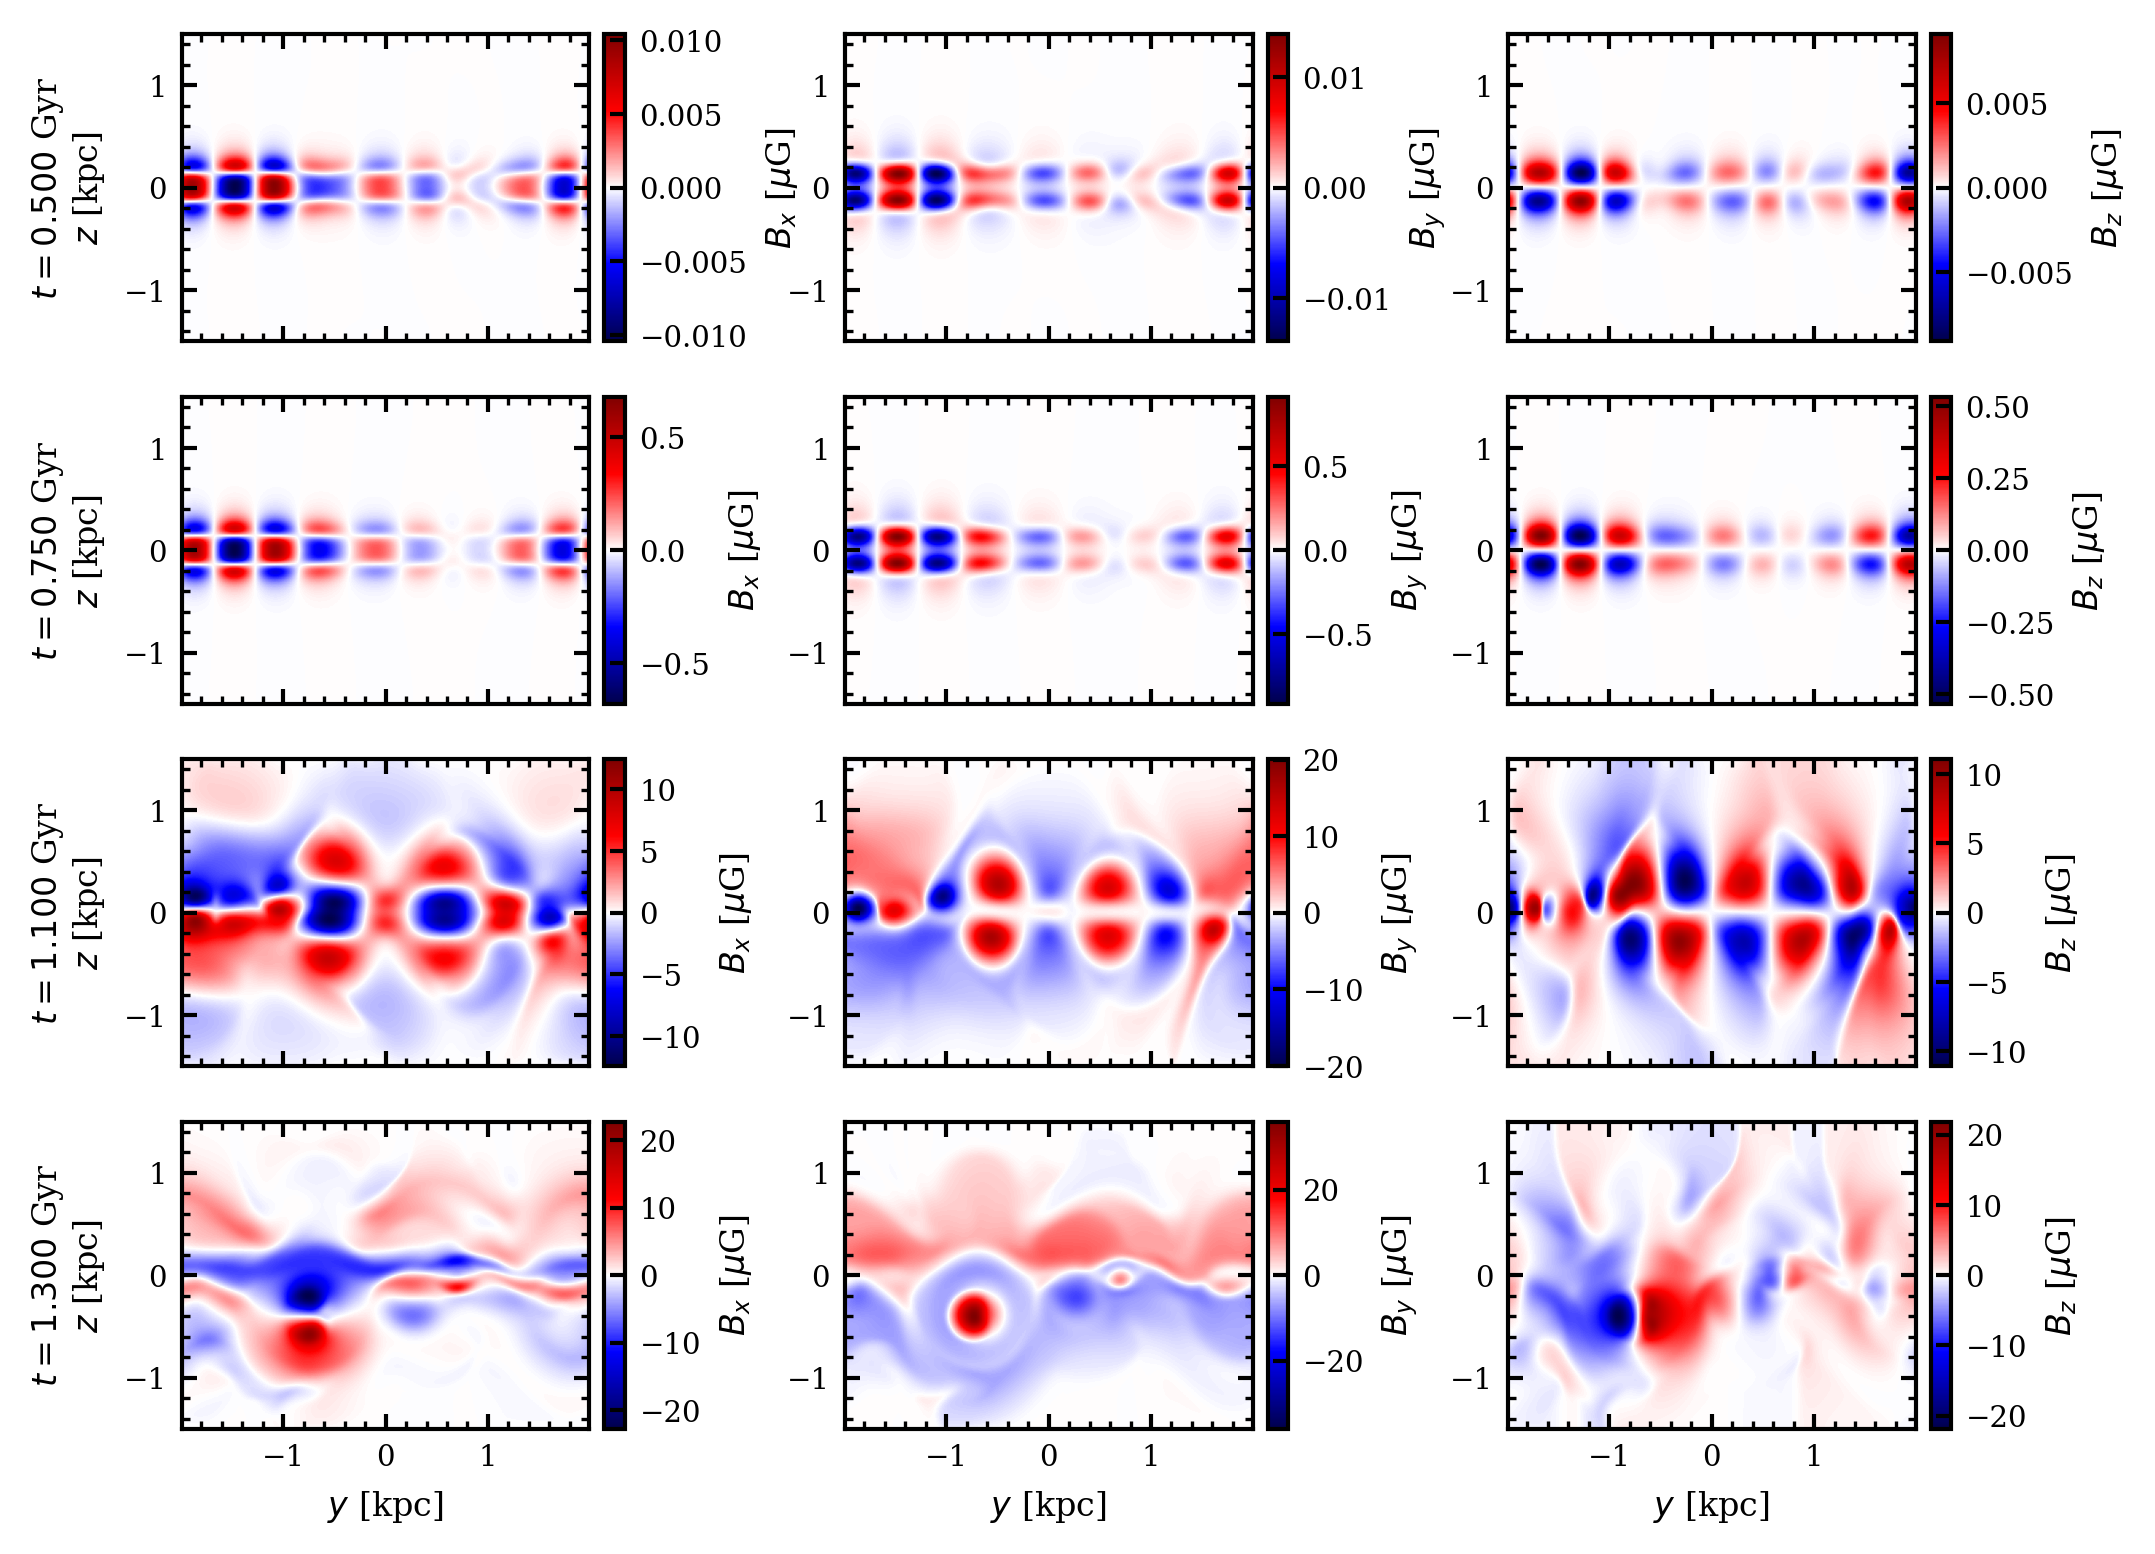
\includegraphics[width=0.8\textwidth]{magnetic_field_evolution.png}
    \caption{The components $\langle B_x\rangle_{xy}$, $\langle
B_y\rangle_{xy}$ and $\langle B_z\rangle_{xy}$ (columns from left to right) in
the (y,z)-plane at various evolutionary stages in Model \RSOBSD.  During the
{linear phase of the (upper row $t = 0.5\Gyr$)} the strength of the magnetic
field grows, while its spatial structure remains largely unchanged (second row,
$t=0.75\Gyr$){, but precipitates the onset of MBI} which  marks the
appearance of large-scale vortical structure in the magnetic field {late in
the linear phase of the MBI} (third row, $t = 1.1\Gyr$). {The non-linear
phase of the MBI saturates with vortical structures spanning $\geq1\kpc$}
(lower row, $t=1.3\Gyr$).  }
    \label{fig:field_evolution}
\end{figure*}
%-----------------------------------------------------------------

In some studies gravitational fields that can be easily incorporated into
analytic solutions have been adopted, many of these only consider the baryonic
disc such as \citet{Giz1993,Luiz_R_2015a}. For these studies, the disc is
modelled as self-gravitating with an iso-thermal velocity dispersion, and its
gravitational field has the form
\begin{equation}
    g(z) = -2\pi G\Sigma \tanh(z/H)
\end{equation}
where $H=500\p$ is the scale height of the disc,
$\Sigma=10^2\rm{M}_{\odot}\p^{-2}$ is the surface density of stars and $G$
Newton's gravitational constant, which applies to the self-gravitating disc.
\citet{LBO2017} suggest an alternative form of this equation which adds a
contribution from the dark matter halo $g_{\rm tot}=g+g_{\rm DM}$ and also
takes into account variations in the gravitational profile with respect to
galactocentric radius.

With a numerical approach, we can adopt more realistic models for the
gravitational field appropriate for the solar vicinity of the Milky Way, which
also includes the contributions from the dark matter halo and takes into
account the large-scale rotation and shear rates. Following
\citet{Ferriere_1998}, we use the gravitational acceleration of
\citet{K&G1989MNRAS} scaled to account for the radial variation of the
gravitational potential,
\begin{equation}
    g =-a_1\frac{{z}}{\sqrt{{z_1}^2+z^2}}\exp{\left(\dfrac{{R_{\odot}-R}}{a_3}\right)} -a_2{\frac{z}{z_2}}\dfrac{R^2_{\odot}+z_3^2}{R^2+z_3^2}
    - 2\Omega(\Omega+S)z\,,
    \label{eq:acceleration}
\end{equation}
where $R_\odot=8.5\kpc$ is the radius of the Solar orbit, $a_1 = 4.4 \times
10^{-14}\km\s^{-2}$ (accounting for the stellar disc), $a_2= 1.7\times 10^{-14}
\km\s^{-2}$ (accounting for the dark matter halo), $z_1=200\p$,/ $z_2=1\kpc$,
$z_3 = 2.2\kpc$ and $a_3 = 4.9\kpc$.  Stronger gravity at smaller $R$ leads to
a thinner gas disc in the initial state and correspondingly smaller values of
$h_\alpha$ defined below. The Milky Way rotation curve of \citet{1985Clemens}
is used in models for the inner parts of the galactic disc.

Although we aim to explore the interaction of the mean-field (turbulent) dynamo
with the MBI and Parker instability, we do not simulate interstellar turbulence
to ease the control and transparency of the model. Instead, we impose the
$\alpha$-effect with parameters typical of spiral galaxies, which drives the
mean-field dynamo action. We use the same form of the $\alpha$-effect as
\cite{QSTGB23}, antisymmetric in $z$, localized around the midplane within a
layer $2h_{\alpha}$ in thickness and smoothly vanishing at larger altitudes,
\begin{equation}
    \label{eq:alpha}
    \alpha(z)=\alpha_0
    \begin{cases}
    \displaystyle
    \sin \left(\pi z/h_\alpha\right)\,, &|z| \leq h_\alpha/2\,,\\
    \displaystyle
    (z/|z|) \exp \left[-\left(2z/h_\alpha-z/|z|\right)^2\right]\,, &|z|>h_\alpha/2\,.
    \end{cases}
\end{equation}
The smaller $h_{\alpha}$, the stronger the vertical gradient of the magnetic
field and the more it is buoyant.  In
Sections~\ref{sec:Rotation}--\ref{sec:emf}, we explore generic features of the
MBI and adopt $h_{\alpha} = 0.3 \kpc$ (equal to the initial density scale
height) to make the instability stronger, this also allows for a more direct
comparison with the case of a non-rotating system \citep{QSTGB23}.

As listed in Table~\ref{tab:sims}, we include several different models which
explore extreme values for $R_{\alpha}$ and $R_\Omega$ in order to discern how
rotation affects the nonlinear phase of the system. {The models {\RAOASA,
\RAOASACM} and {\RBOASACM} consider different galactocentric distances}.
{\RBOASACM\ uses parameters which match M31} at $R=3\kpc$. We adopt the
magnitude of the $\alpha$-effect $\alpha_0 = 2.25 \kms$ (e.g., p.317 of
\citealt{SS21}).

The dynamo intensity (both the rate of exponential growth of the magnetic field
strength at an early stage and its steady-state magnitude) depends on the
dimensionless parameters
\begin{equation}\label{Ral}
R_\alpha=\alpha_0 h_\alpha/\eta\quad \text{and} \quad   R_\omega=Sh_\alpha^2/\eta\,,
\end{equation}
which quantify the magnetic induction by the $\alpha$-effect and differential
rotation, respectively. When $R_{\alpha} \ll |R_\omega|$, the magnetic field is
mostly sensitive to their product known as the dynamo number,
\begin{equation}\label{DynNum}
     D=R_\alpha R_\omega\,.
\end{equation}

\citet{QSTGB23} considered a non-rotating system with an imposed
$\alpha$-effect, a form of the mean-field dynamo known as the
$\alpha^2$-dynamo. Here we include differential rotation to obtain a stronger
magnetic field amplification mechanism, the $\alpha^2\Omega$-dynamo.

\begin{figure*}%---------------------------------------------------------------------
    \centering
    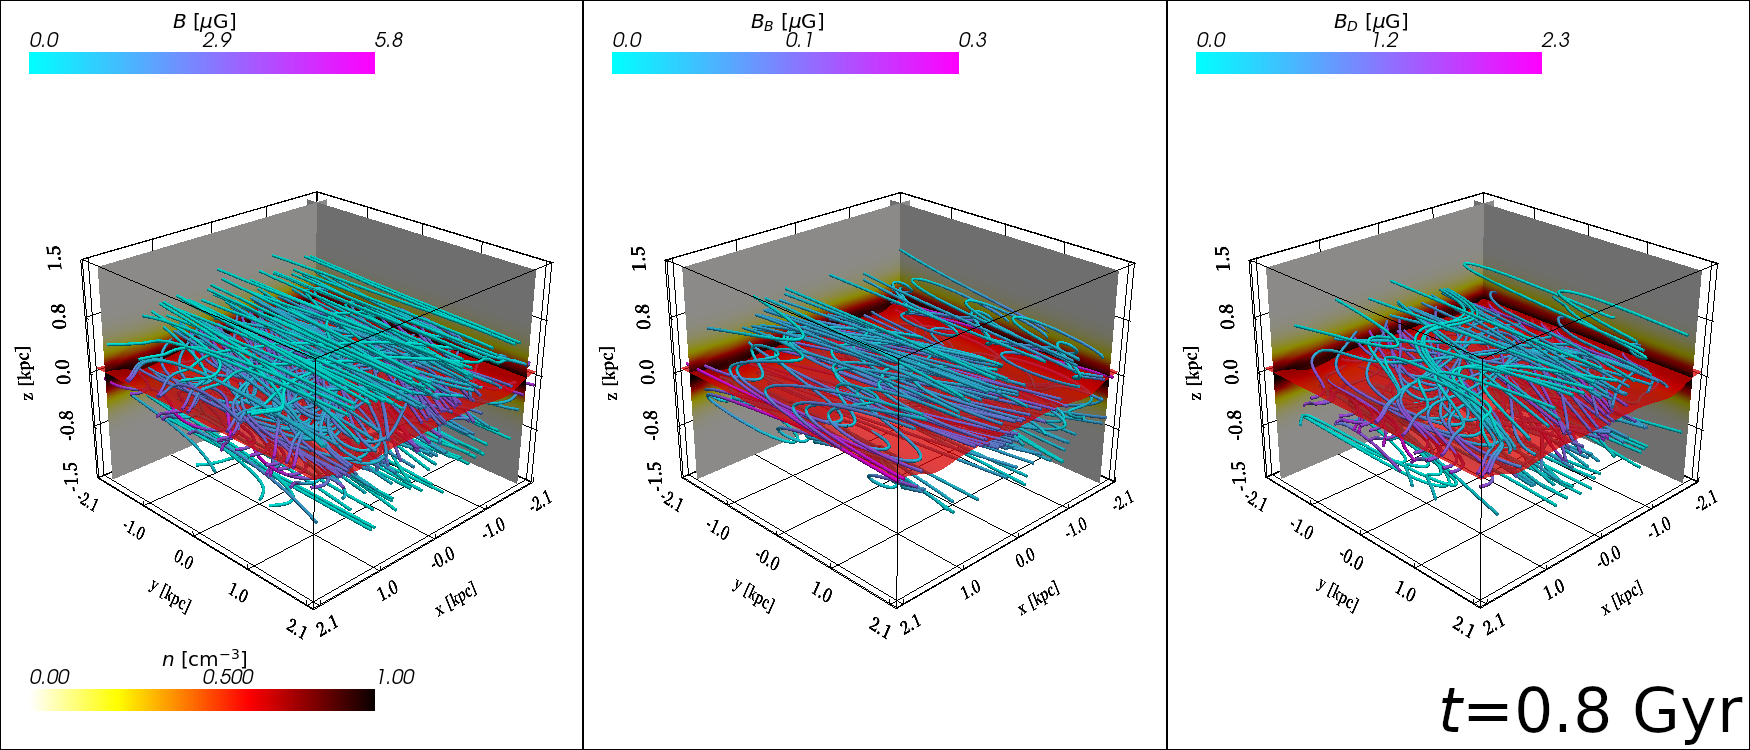
\includegraphics[trim=0.0cm 0.0cm -23.9cm 0.0cm,clip=true,width=1\textwidth]{3d_streamlines_t08.png}\\
    %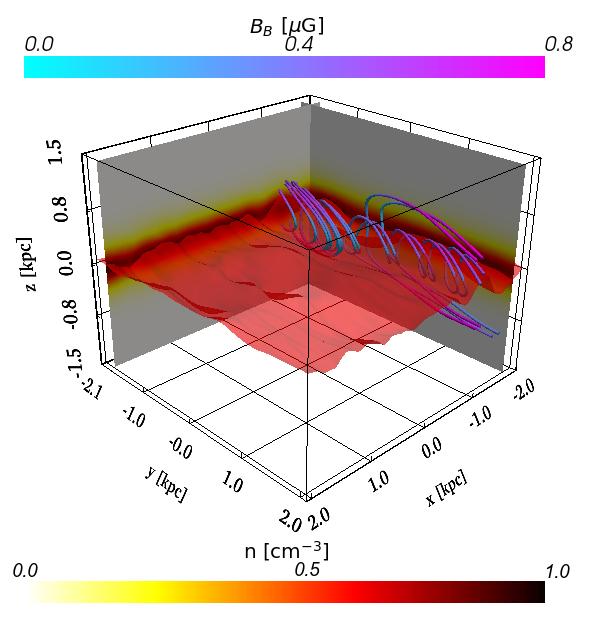
\includegraphics[width=0.28\textwidth]{parker_loops.png}
    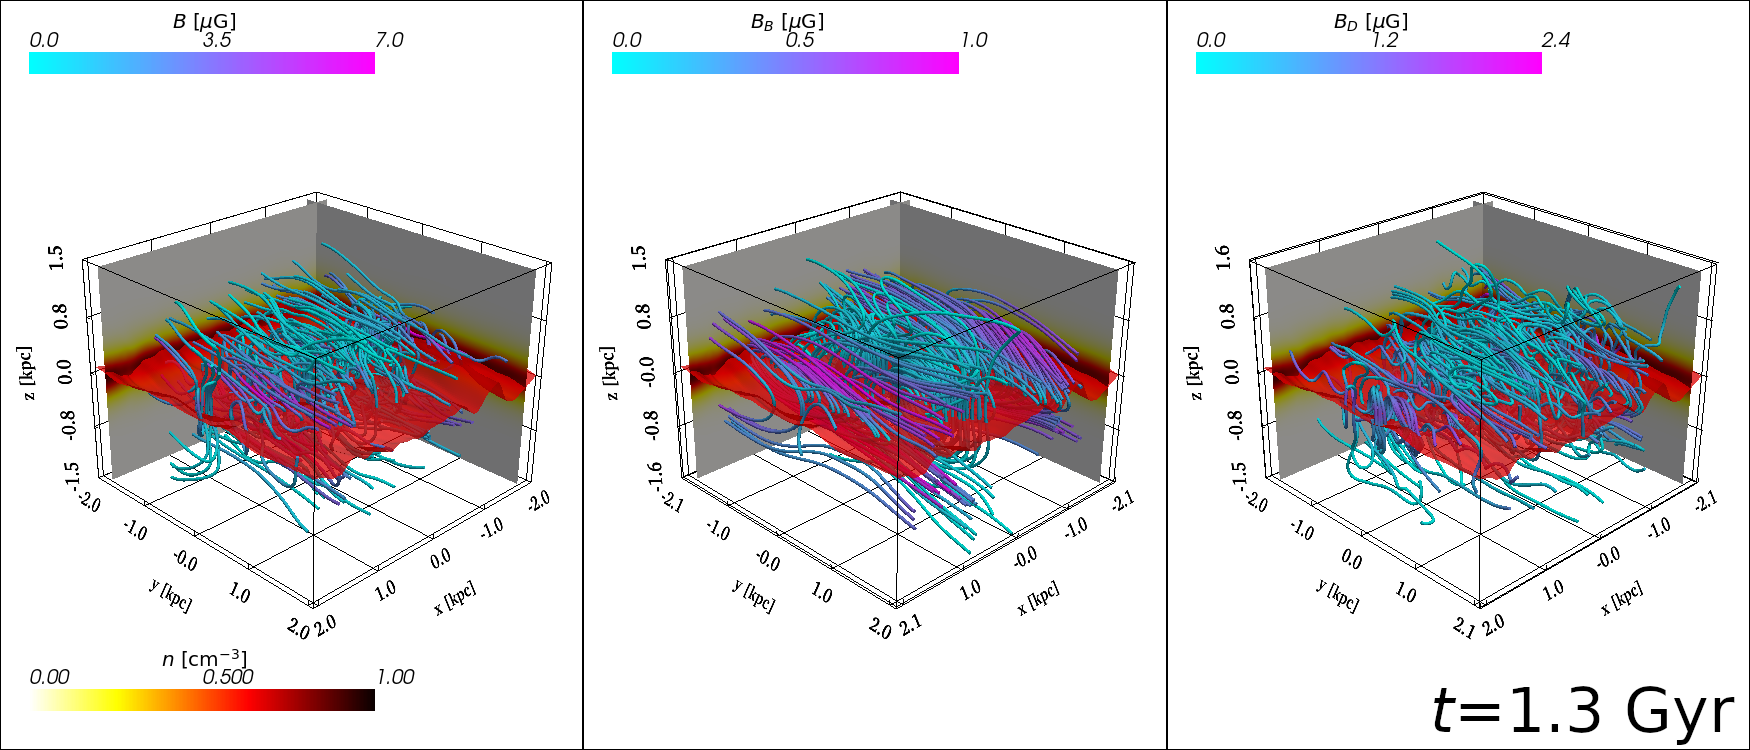
\includegraphics[width=0.72\textwidth]{3d_streamlines_t13.png}
    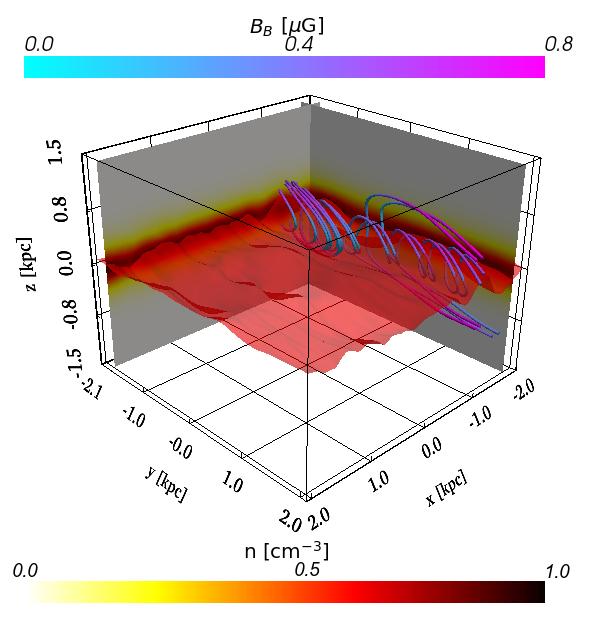
\includegraphics[trim=0.0cm -2.0cm 0.0cm 0.0cm,clip=true,width=0.27\textwidth]{parker_loops.png}
    \caption{The field lines in Model {\RSOBSD} of the total magnetic field
$\BB$ (left hand column) are separated using a Gaussian kernel of smoothing
length $\ell=200\p$ into contributions characteristic of the magnetic buoyancy
$\BB_\text{B}$ with the larger scales (middle) and those of the imposed dynamo
$\BB_\text{D}$ exhibiting smaller scales (right-hand column). The red
isosurface maps onto the gas number density at $0.7\cm^{-3}$.
\label{fig:streamlines} \label{fig:loops} Portion {(offset)} of the
mean-field $\BB_\text{B}$ taken from {lower row, second panel} where the
Parker loops are easily identifiable.}
\end{figure*}%---------------------------------------------------------------------

%---------------------------------------------------------------------
\section{Results}\label{sec:Results}

{For reference we examine Model}
\RSOBSD\
{(see
Table~\ref{tab:sims}), referring to other models in respect of detailed
effects.} Models {\RVOASA} and {\RXOASA} use Prantdl numbers matching those
with $\Omega=0$ of \citet{QSTGB23} in order to isolate the effects of rotation.
The runs \RSOBSA --\RSOBSE\ are used to explore how rotation affects the final
steady state parity, while models {\RAOASA, \RAOASACM\ and \RBOASACM} use
parameters which reflect various galactocentric radii with values adopted from
the rotation curve for the Milky Way of \citet{1985Clemens}.

%---------------------------------------------------------------------
\subsection{{The evolution of both} dynamo and magnetic buoyancy}\label{sec:Rotation}

The system explored supports the mean-field $\alpha^2\Omega$-dynamo and the
magnetic buoyancy instabilities.  The main features of the interaction of the
dynamo and MBI can be illustrated using Model \RSOBSD\ in which their growth
rates and characteristic scales are quite different. Since $|R_\omega|\approx
R_\alpha$ in this model, the estimate of the dynamo length scale of about
$h_\alpha=300\p$ obtained by \citet[][section~3]{QSTGB23} remains a valid
approximation; the wavelength of the MBI is much larger, of order 1--2\,kpc.
{This separation is supported by an inspection of the evolving field
structure evident in Figure~\ref{fig:field_evolution}.}

%--------------------------------------------------------------------------------------
\begin{figure*}
    \centering
    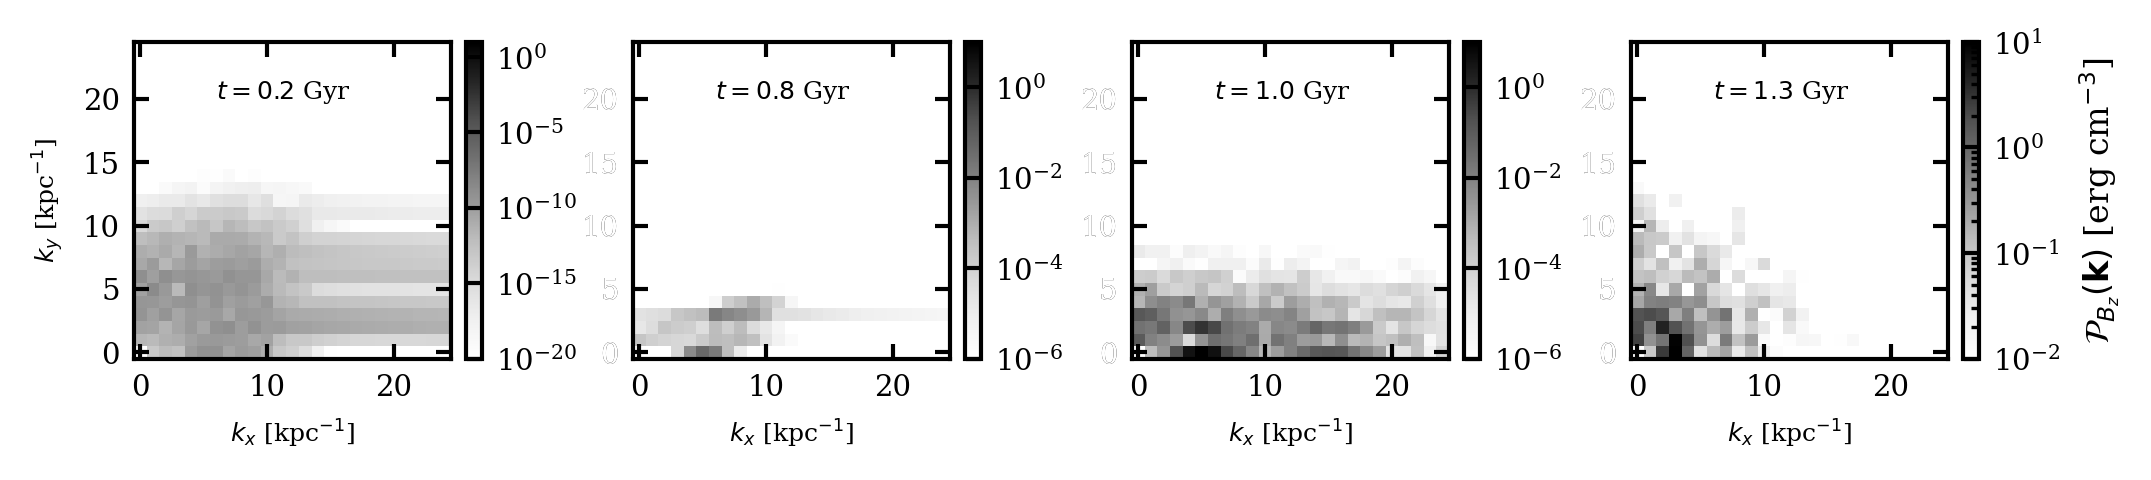
\includegraphics[width=\textwidth]{power_spec.png}
    \caption{Two-dimensional power spectra in the ($k_x$,$k_y$)-plane of $B_z$
in Model \RSOBSD\ at $z=385\p$ during the evolution of the mean-field dynamo
and onset of the MBI (leftmost and middle panels) through to a stationary
state (right).}
    \label{fig:Power_spec}
\end{figure*}
%--------------------------------------------------------------------------------------

At early times (upper row), magnetic field produced by the dynamo at a
relatively small scale is too weak to be buoyant, but, as its strength
increases, it {becomes susceptible to distortion} by magnetic buoyancy
(second row).  The spatial structure dominated by the MBI is shown in the third
row corresponding to the time when the system enters the stationary state. Here
the magnetic field has spread to large altitudes and the vertical magnetic
field has become locally comparable in magnitude to the horizontal {field}
components. The vertical parity of the magnetic field remains quadrupolar (the
same as in the dynamo field): the horizontal field is symmetric with respect to
the plane $z=0$ while the vertical field is antisymmetric. Despite the strong
difference in the spatial scales, this structure is maintained by the dynamo
action, this is a true symbiosis of the two processes.

The evolution described above is quite similar to that discussed by
\citet{QSTGB23}, where $\Omega=0$ and $S=0${, but yields} enhanced regular
magnetic patterns at $t\leq1.1\Gyr$, {due to the stronger shear dynamo
action}.  {Compare these first three rows} with figure~4 of \citet{QSTGB23}
where the evolution is slower and the magnetic structures are less regular
because of a weaker dynamo. However, thus far this has not introduced any
qualitative changes into the system.

This difference {in the characteristic scales motivates} us to separate the
two types of the magnetic field using the Gaussian smoothing \citep{Gent2013}.
The buoyancy-driven part is obtained from the total magnetic field
$\vec{B}(\vec{x},t)$ as
\begin{equation}\label{GS}
    \BB_\text{B}(\vec{x},t) = \int_{V}B(\vec{x}^\prime,t)\,G_{\ell}(\vec{x}-\vec{x}^\prime)\,\dd^3\vec{x}^\prime\,,
\end{equation}
where the integration extends over the whole domain volume with the smoothing
kernel $G_\ell(\vec{\zeta}) =
(2\pi\ell^2)^{-3/2}\exp{[-|\vec{\zeta}|^2/(2\ell^2)}]$ and $\ell =
200\text{--}300\p$ chosen to be close to the dynamo scale $h_\alpha$. The
remaining part of the magnetic field $\vec{B}\D = \vec{B}-\vec{B}_\text{B}$ has
scales smaller than $\ell$. It is mostly due to the dynamo action but also
contains random fields produced by nonlinear effects at the later stages of the
system's evolution.

{Applying this filter we} illustrate {in Figure~\ref{fig:streamlines}}
the {3D} field structures, including the prominent loops produced by the MBI
and the magnetic field generated by the dynamo transformed by the MBI.
{Magnetic field lines are plotted (left to right) for the total field,
$\BB$, the buoyancy-driven field $\BB_\text{B}$ and the dynamo field
$\vec{B}\D$, before the growth of the MBI at $t=1\Gyr$ and after it has
saturated at $t=1.3\Gyr$.} The instability produces buoyant loops of a
large-scale magnetic field at a kiloparsec scale. These `Parker loops' are
expected to lie largely in the azimuthal direction, the direction of the
large-scale field.  This corresponds to the `undular' modes (with wavevector
parallel to the magnetic field $\BB$), which are expected to dominate over the
`interchange' modes (with wavevector perpendicular to $\BB$), derived from
linear analyses of the instability \citep[see, e.g.,][]{MTSK1993}. Such twisted
loops are seen offset in Figure~\ref{fig:loops} which displays a small portion
of the mean-field in the nonlinear stages of the system. These loops suggest
possible observational signatures of the instability which may present in
rotation measures or polarized synchrotron intensity maps. A more in-depth
discussion of these observational signatures is explored by
\citet{Luiz_R_2015a}.

{To help quantify the changes to the system we can measure the spectra and
the growth of the magnetic field.} The restructuring of the magnetic field of
model \RSOBSD\ by the MBI is quantified in Figure~\ref{fig:Power_spec}. This
shows the two-dimensional power spectra of the $z$-component of the magnetic
field at times indicated.  These confirm the evolution pattern visible in
Figure~\ref{fig:field_evolution}. Over time the dominant horizontal scales
$2\pi k_x^{-1}$ and $2\pi k_y^{-1}$ of the magnetic field grow larger.  At
$t\lesssim 0.2$ the energy is {already} confined to azimuthal scales
$k_y\lesssim 10\kpc^{-1}$, {while} radial scales extend to
$k_x>20\kpc^{-1}$. This is in agreement with the analysis of \citet{S1974}, as
the dominant azimuthal wavenumber $k_y$ decreases under the influence of
rotation. The dominant horizontal scales reduce through to $t=1.3\Gyr$ to reach
$k_x\approx 4$ and $k_y\approx 2$.  These wavenumbers correspond to scales of
$1-2\kpc$ which are the characteristic scales of the MBI.  The dynamo saturates
at large scales, and with a narrowing spectrum ($t=0.8\Gyr$). As the peak
wavenumbers decrease further, due to the onset of MBI, their spread is broader,
as the MBI excites a wider range of unstable modes.

%-----------------------------------------------------------------
\begin{figure}
    \centering
    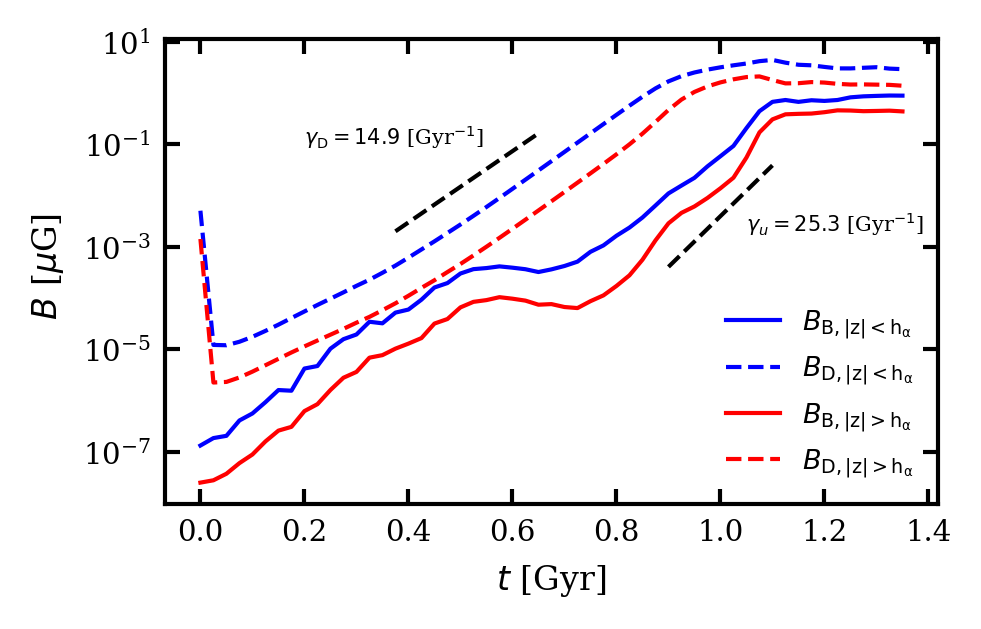
\includegraphics[width=0.45\textwidth]{Mag_in_out.png}
    \caption{The evolving magnitude of the magnetic field in model \RSOBSD\ at
large-(solid) and small-scale (dashed), using scale separation
$\ell=\fg{3}00\p$, averaged over $\lvert z \rvert < h_{\alpha}$ (blue) and
$\lvert z \rvert > h_{\alpha}$ (red).  Dashed lines (black) indicate the
exponential growth at the rates presented in Table~\ref{tab:sims}.
    }
    \label{fig:ts_mag}
\end{figure}
%-----------------------------------------------------------------

To {investigate} the growth {rates of the instabilities,} the magnetic
field of is separated into $\BB_\text{B}$ and $\BB_\text{D}$ within and without
$h_\alpha$ of the midplane.  After the initial {turbulent transient decay,
the total} field strength {in time up to} a stationary state.  {This rate
of growth $\gamma_\text{D}$ of the total field within $|z|\leq h_\alpha$ for
each model in Table~\ref{tab:sims} is fitted at a time once its strength
recovers \fg{10} times its minimum through to \fg{5\%} of its maximum.  In the case of
Model \RSOBSD\ this spans \fg{$0.2\Gyr\lesssim t \lesssim0.75\Gyr$} and is
identified in Figure~\ref{fig:ts_mag} with $\gamma_\text{D}=\fg{17.5}\Gyr^{-1}$.}

{Once the field becomes buoyant it induces an instability in the velocity
field, which grows exponentialy. In all models this growth rate
$\gamma_\text{u}$ is fitted at times once $u_\text{rms}$ exceeds \fg{10} times its
minimum through to \fg{10\%} of its maximum. This is indicated for Model \RSOBSD\ in
Figure~\ref{fig:ts_mag} as $\gamma_\text{u}=\fg{34.5}\Gyr^{-1}$ spanning
\fg{$0.75\Gyr\lesssim t \lesssim 1\Gyr$.}}

{In Figure~\ref{fig:ts_mag}} the small{-scale field} $\BB_\text{D}$
(dashed blue), {mainly driven} by the dynamo action {has a near constant
growth rate through to} the stationary state at $t\simeq\fg{1.1}\Gyr$. Dynamo action
is localized at {$|z|\lesssim h_\alpha$}, but the magnetic field spreads
diffusively to larger altitudes (dashed red) where, although much weaker,
{it has} the same {growth} rate.  {At $t\lesssim\fg{0.5}\Gyr$ the
large-scale field} $\BB_\text{B}$ (solid lines) represents just the large-scale
tail of the leading dynamo eigenfunction.  {However, its behaviour
subsequently changes dramatically, stagnating some \fg{200} Myr, while
$\BB_\text{D}$ continues to grow.}

{This transition is not observed when differential rotation is absent in
\citet{QSTGB23} where instead $\BB_\text{B}$ growth exceeds that of
$\BB_\text{D}$ once MBI is excited. Here, following the transition MBI exerts a
new dynamo action on $\BB_\text{B}$ but only at a rate similar to
$\gamma_\text{D}$.  The transitory stagnation in $\BB_\text{B}$ growth, may be
due to the horizontal shear suppressing the vertical scales in the magnetic
field and tangling them into smaller structures along the horizontal plane,
which is reflected in the growth of small scale structure in $k_x$ between 0.8
and 1 Gyr in Figure~\ref{fig:Power_spec}, but not in the direction of shear
$k_y$. The tangling effect of shear on the Parker loops is also a feasible
explanation for the reduced growth rate of $\BB_\text{B}$ during the
MBI.\footnote{\fag{Need to check the numbers referring to Figure 4 once the
plot is reverted}}}

%---------------------------------------------------------------------
\subsection{Effect of parameters on growth rates.}\label{sec:params}

{The perturbations corresponding to the $\alpha^2\Omega$-dynamo and the MBI}
grow exponentially during their linear stages at different rates, becoming
strongly intertwined during nonlinear stages of the instability when the
Lorentz force becomes dynamically significant and the system evolves into a
stationary state.  The two processes respond differently to the system
parameters.  For example, reducing {only} $h_\alpha$ makes the dynamo action
weaker, because the dynamo parameters $R_\alpha$ and $R_\omega$ become smaller,
but enhances the MBI, because the gradient of the magnetic field strength
increases with ${h_\alpha}^{-1}$.  Furthermore, the MBI is sensitive to both
the magnetic diffusivity and the kinematic viscosity whereas the dynamo action
is relatively insensitive to the kinematic viscosity.

The {parameters and outcomes} presented in Table~\ref{tab:sims} are designed
to {aid identification of the} physical processes responsible for salient
features of the {system} steady-state.  Some unrealistic parameter values
{have been} chosen to enhance the difference in the properties of the dynamo
and MBI. We flag such parameter choices and emphasise results {that} were
obtained for the parameter values typical of spiral galaxies.\footnote{
\fag{Here needs to be a paragraph discussion of parameter effects on the growth
rates. Deferred until Table values are confirmed.}}

%---------------------------------------------------------------------
\subsection{Effect of parameters of non-linear field parity}\label{sec:parity}


\begin{figure}%---------------------------------------------------------------------
    \centering
    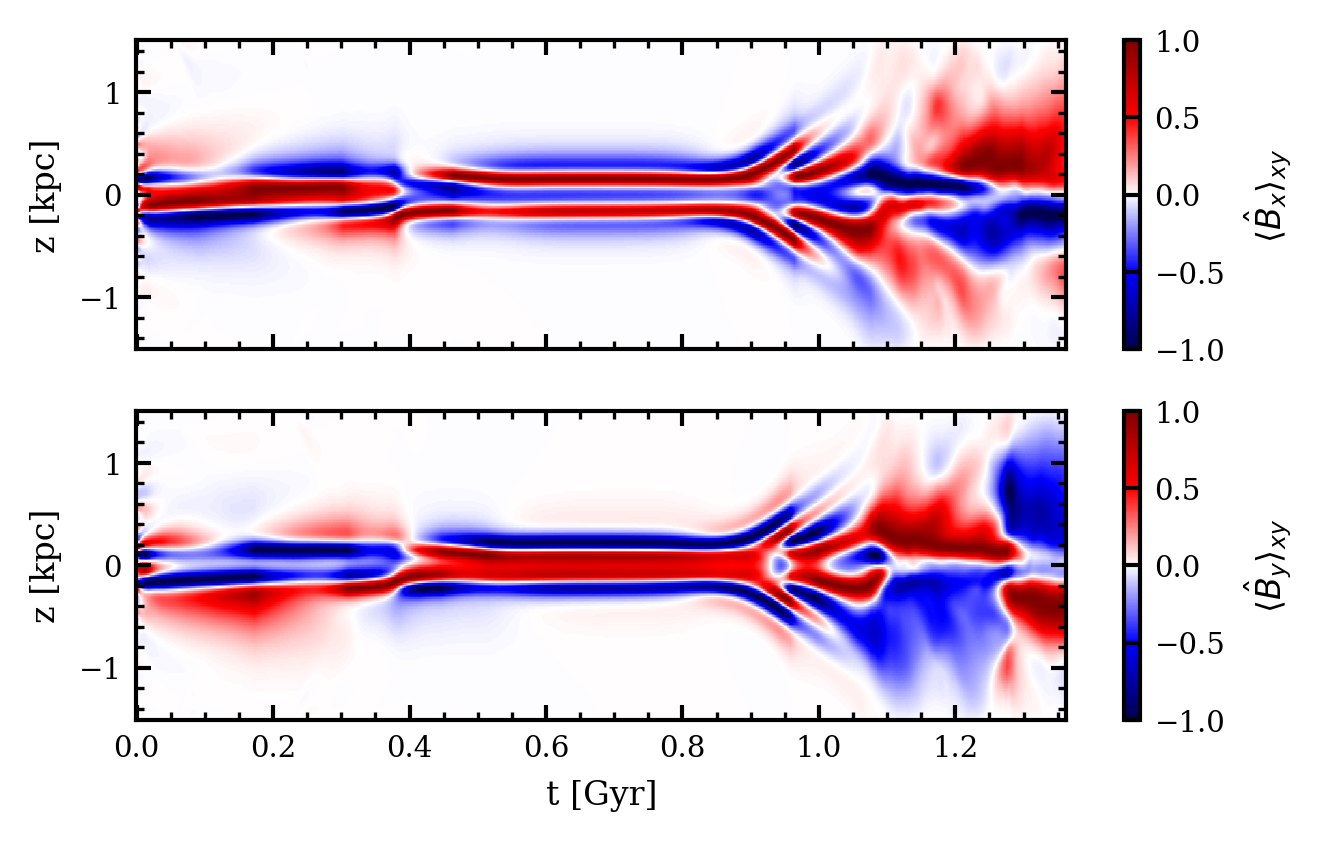
\includegraphics[width=0.52\textwidth]{Ra5h3.png}
    \caption{The evolution of the horizontally averaged magnetic field
components $\langle\widehat{B_x}\rangle_{xy}$ (upper panel) and
$\langle\widehat{B_y}\rangle_{xy}$ (lower panel) in Model {\RSOBSD}.  The hat
indicates that each component has been normalized to its maximum magnitude at
each time.}
    \label{fig:xy_averages}
\end{figure}%---------------------------------------------------------------------

A fundamentally new consequence of the overall rotation emerges at the late
nonlinear stage represented in the fourth row of
Figure~\ref{fig:field_evolution} {in contrast to \citet{QSTGB23}.  T}he
magnetic field changes {to a predominantly dipolar parity}, with
antisymmetric horizontal field components and symmetric vertical field:
{\begin{align}
B_x|_{z<0}&\approx-B_x|_{z>0},\nonumber\\
B_y|_{z<0}&\approx-B_y|_{z>0}\nonumber\\
 &\text{and}\nonumber\\
B_z|_{z<0}&\approx B_z|_{z>0},
\end{align}
}although the
symmetry plane is not flat but rather {undulates at} $z=0$. {The parity
switch occurs} despite the fact that the imposed $\alpha$-effect, confined to
relatively thin layer is expected to continue maintaining a magnetic field of
quadrupolar parity and the buoyancy does not change that in the early nonlinear
stage.  The nature of the parity change is unexpected{.}

Figure~\ref{fig:xy_averages} further illustrates how the parity of the magnetic
field is transformed as a consequence of the MBI under the effects of rotation.
Throughout the dynamo and linear stage of the MBI the magnetic field grows
monotonically before changing parity at $t\geq 1.1\Gyr$ when it becomes strong
enough to make the system essentially nonlinear. The figure shows the evolution
of the horizontally averaged magnetic field components $\langle
B_x\rangle_{xy}$ and $\langle B_y\rangle_{xy}$ from Model~\RSOBSD, normalized
to their maximum values at each time to better expose the field structure at
early times when it is still weak.

Models {\RVOASA} and {\RXOASA} use parameters from the simulations R5h2 and
R10h2 in \citet{QSTGB23}. None of those models without rotation exhibit this
change of parity. Model {\RXOASA} is very similar to R10h2 with exponential
growth in the linear phase that gives way to oscillations in the nonlinear
phase. However, model {\RVOASA}, which has a weaker imposed $\alpha$-effect,
displays a change in parity in the nonlinear phase which is not present in
{\RXOASA}. The trend seen in models {\RSOBSA}-{\RSOBSE} implies the change in
parity occurs when the $R_\omega$ is comparatively smaller than $R_\alpha$.
{This would also indicate that increasing the} dynamo scale height
$h_{\alpha}$ encourages the formation of a magnetic field with dipolar parity.
{Such fields} are generated preferentially within spherical geometries and
thick discs.

Observational evidence {exists} for magnetic fields with non-axisymmetric
components, most notably M81 \citep{KBH1989,SSK1992}.  Results on the all-sky
distribution of rotation measure (RM) {\citep{TSS2009} found some}
line-of-sight magnetic fields are largely consistent with dipole-like models in
which azimuthal magnetic fields are antisymmetric relative to the midplane.
However, small-scale variations in the RM distribution, influenced by the
turbulent structure of the gas in the disk, add complexity to these
observations. \citet{BHB2010} observed RM distributions in nearby galaxies and
also noted that the magnetic field topology of the upper halo of galaxies is a
mixture of dipolar and quadrupolar structures in thick discs and radially
directed dipolar fields in halos. \citet{XH2024} also reached similar
conclusions with RM measurements of the Galactic halo and find signs of a
regular dipolar magnetic field.  Faraday rotation measures (RMs) of the regular
fields in halos from the CHANG-ES data \citep{CHANG-ES2024} reveal no
preference for clear simple symmetry having neither preference for purely
quadrupolar or dipolar field structures.

 {With theoretical approaches} \citet{RWBM1990} and \citet{MTB1991} have
investigated nonlinear spherical mean-field dynamo models in which stable
nonaxisymmetric fields may be excited with suitably chosen distributions of
alpha effect and differential rotation \citep[see also][]{S1971}.
\citet{RE1992} considered models where the introduction of anisotropy in the
alpha tensor may have a similar effect \citep[see also][]{R1980}. However, when
constructing galactic dynamo models, there is less freedom, as the differential
rotation is then known and cannot be chosen in an arbitrary manner. In general
differential rotation is known to discriminate against the excitation of
nonaxisymmetric  dynamo modes compared with axisymmetric, although this effect
is very much reduced in thin disc geometry \citep{MB1992}. However, galactic
mean-field dynamo models with axisymmetric distributions of $\alpha$-effect and
turbulent resistivity have not been found preferentially to excite
nonaxisymmetric fields.

Simulations by \citet{MNKASM2013} investigate a system which included the
magneto rotational instability and the Parker instabilitys. Their figure~6
shows clear regular reversals similar to those found in \citet{QSTGB23}.
Furthermore, figure~10 of \citet{MNKASM2013} shows the distribution of RM
obtained from their numerical results which correspond to a dipolar magnetic
field. {Simulations of galactic dynamo, applying supernova-driven turbulence
however, so far show solutions which are quadrupolar
\citep{Gressel2008,OGPhD,Gent2013,GMK23}, but have been restricted to solar
neighbourhood parameters.}

\subsection{The effect of cosmic rays}\label{sec:CM}

We model cosmic rays in a way similar to \citet{DT2022b} and
\citet{Luiz_R_2015a} using a fluid approximation (e.g. \citet{Parker1969};
\citet{SRLI1985}) where the cosmic ray energy density $\epsilon_{cr}$ is
governed by
\begin{equation}
    \deriv{\epsilon_\text{cr}}{t} + \nabla\cdot(\epsilon_\text{cr}\vec{u}) + p_\text{cr}\nabla\cdot\vec{u} + \mathcal{Q}(z) =  -\nabla \cdot\vec{F}\,,
\end{equation}
with $\vec{F}$ the cosmic ray flux defined below and $\mathcal{Q}(z)$ a source term with the form
\begin{equation}
    \mathcal{Q}(z) = \epsilon_\text{cr,0}\exp(-|z|^2/h_\text{cr}^2)\,.
\end{equation}
The source term is chosen to replicate the injection of cosmic rays into the
ISM by supernovae. The typical supernovae explosion (SNe) ejects a mass with
$M_{ej}$ with a kinetic energy $E_0 = 10^{51}\erg$, roughly $10\%$ of the
energy is converted into cosmic ray energy, these SNe are expected to occur
within a roughly $100\p$ disc. To replicate this situation we choose the scale
height of the energy injection to be $h_{cr}=100\p$ and $\epsilon_{cr,0} =
10^{50}$.

\begin{figure}
    \centering
    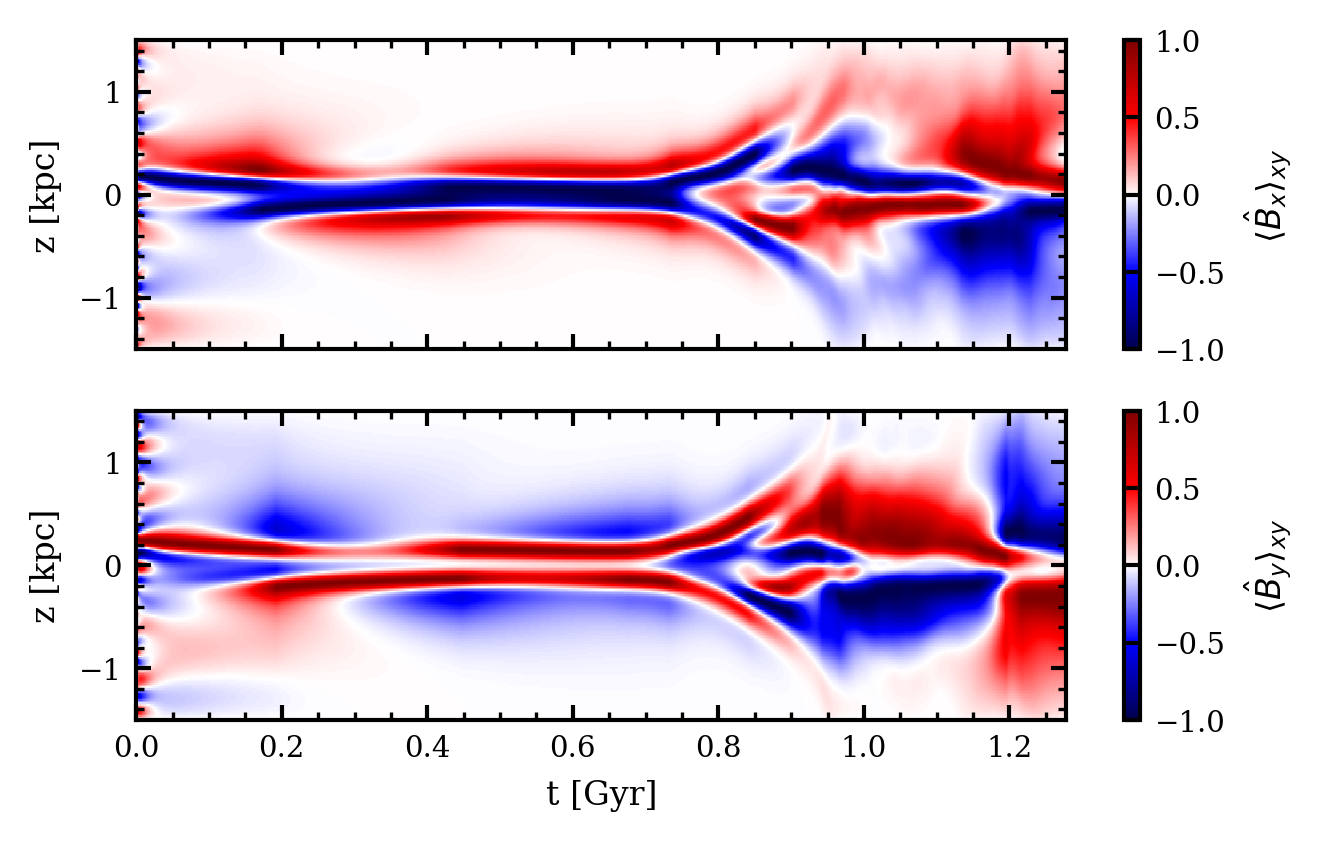
\includegraphics[width=0.5\textwidth]{1D_xy_aver_cm.png}
    \caption{Horizontal averages of the horizontal components of the magnetic field $\langle \widehat{B}_x \rangle_{xy}$, $\langle \widehat{B}_y \rangle_{xy}$ in Model~\CM.}
    \label{fig:xy_aver_cm}
\end{figure}

Figure~\ref{fig:xy_aver_cm} presents the horizontal averages for the Model~\CM,
including cosmic rays. Cosmic rays exert considerable pressure and have
negligible weight, enhancing the effects of magnetic buoyancy and subsequently
making the dynamo and instability stronger. The trend evident from the results
listed in %of Table~\ref{tab:sims} suggests that stronger buoyancy would cause
the field parity in the nonlinear stages of the system to be quadrupolar and
this is true for the typical dynamo numbers around the solar neighbourhood are
$R_{\alpha}\simeq 0.5$ and $R_{\Omega}\simeq -15$, models {\RAOASA} and
{\RAOASACM} adopt these parameters.  The early stages of the evolution for
model~{\RAOASA} are uneventful with the imposed $\alpha$-effect amplifying the
magnetic field in the linear stage of the instability ($t<5.5$Gyr) and then in
the nonlinear stages of the instability ($t>5.5$Gyr) the magnetic field spreads
out away from the disc and has a quadrupolar field parity. Models~{\RAOASACM}
and {\RBOASACM} which include cosmic rays, with the latter using parameters
that represent the galaxy at the galactocentric radius $R=3\kpc$, both have
even parities in their nonlinear phases.

\section{Interpretation of results}\label{sec:interp}

All models follow a similar linear evolution of exponential magnetic energy
growth arising from the combined effects of the imposed $\alpha$-effect and the
$\Omega$-effect due to the galactic shear. Once the magnetic field is strong
enough to become dynamically significant there is exponential growth of the
r.m.s velocity. As the kinetic and magnetic energies reach equipartition the
magnetic field saturates and the system enters its nonlinear phase, at which
point the resultant field structures become vastly different. The magnetic
field generated by the linear dynamo is confined to a relatively thin layer,
$\lvert z \rvert \lesssim h_{\alpha}$ and grows monotonically. However, after
inducing the MBI it spreads to larger altitudes through buoyancy to acquire
scale height of order $1\kpc$.  When fully nonlinear the magnetic field
undergoes a dramatic change in structure from an initially quadrupolar field
structure to a now dipolar field structure in simulations \RSOBSB-\RSOBSE.
Model {\RSOBSA} has a higher rate of shear than these other models and does not
display the same change in parity. Differential rotation is known to suppress
the excitation of non-axisymmetric modes which may explain why this model does
not display the same change in parity.


To understand how the presence of large-scale shear can induce such parity
variation and what is the role of the MBI, we can consider the mean field
induction equation, written in terms of $\aver{\vec{B}}$  as
\begin{equation}
    \deriv{\aver{\BB}}{t} = \nabla \times (\aver{\uu})\times \aver{\BB} +\vec{\varepsilon} -\eta\nabla\times\aver{\BB},
\end{equation}
where $\varepsilon$ contributes the electromotive force (EMF) from averaging of
the turbulent fluctuations $\aver{\uu\times\BB^\prime}$. Applying a
second-order correlation approximation to inhomogeneous, anisotropic turbulence
as found in the ISM of a spiral galaxy, a general expression for the EMF has
the form
\begin{align}
    \vec{\mathcal{E}} &= \vec{\upalpha}\cdot\aver{\BB} + \vec{\gamma}\times\aver{\BB} - \vec{\upbeta}\cdot\left(\nabla \times \aver{\BB}\right)  \nonumber\\
    &- \vec{\delta}\times(\nabla\times\aver{\BB}) - \vec{\upkappa}\cdot(\nabla\aver{\BB})^{(s)}\,,
\end{align}
in which tensors $\vec{\upalpha}$ and $\vec{\upbeta}$ are second order and
$\vec{\kappa}$ is third order. Each of these terms represents a physical
process. The $\vec{\upalpha}$ tensor applies effects from small-scale helicity,
$\vec{\upbeta}$ turbulent diffusivity, $\vec{\delta}$ turbulent pumping,
$\vec{\gamma}$ shear or rotating current effects, and $\vec{\upkappa}$ includes
the residual effects, depending on the symmetric part of the magnetic gradient
tensor $(\nabla\aver{\BB})^{(s)}$. A comprehensive study of each of these
effects will be required to explain fully the mean-field dynamo, but we focus
on $\vec{\upalpha}$.

%---------------------------------------------------------------------
\begin{figure}
    \centering
    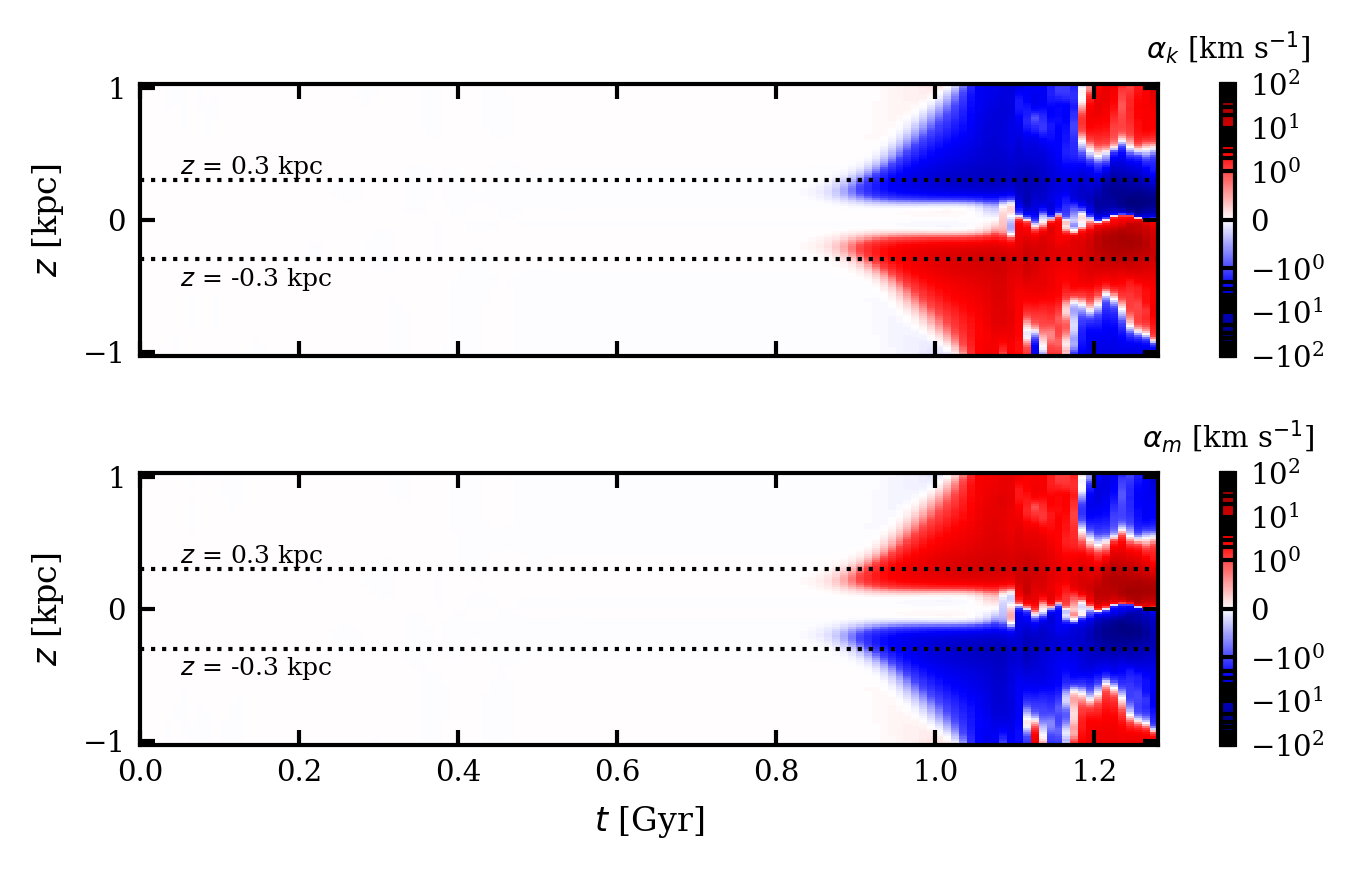
\includegraphics[width=0.5\textwidth]{ak_am.png}
    \caption{The evolution of the horizontally averaged mean kinetic helicity (upper panel) and mean magnetic helicity (lower panel) coefficients of the random velocity and magnetic fields, equations~\ref{alpha_k} and \ref{alpha_m} respectively, in Model \RSOBSD. The horizontal dotted lines are shown at $\lvert z \rvert = h_{\alpha}$.}
    \label{fig:ak_am}
\end{figure}
%---------------------------------------------------------------------

%--------------------------------------------------------------------------------
\begin{figure*}
    \centering
    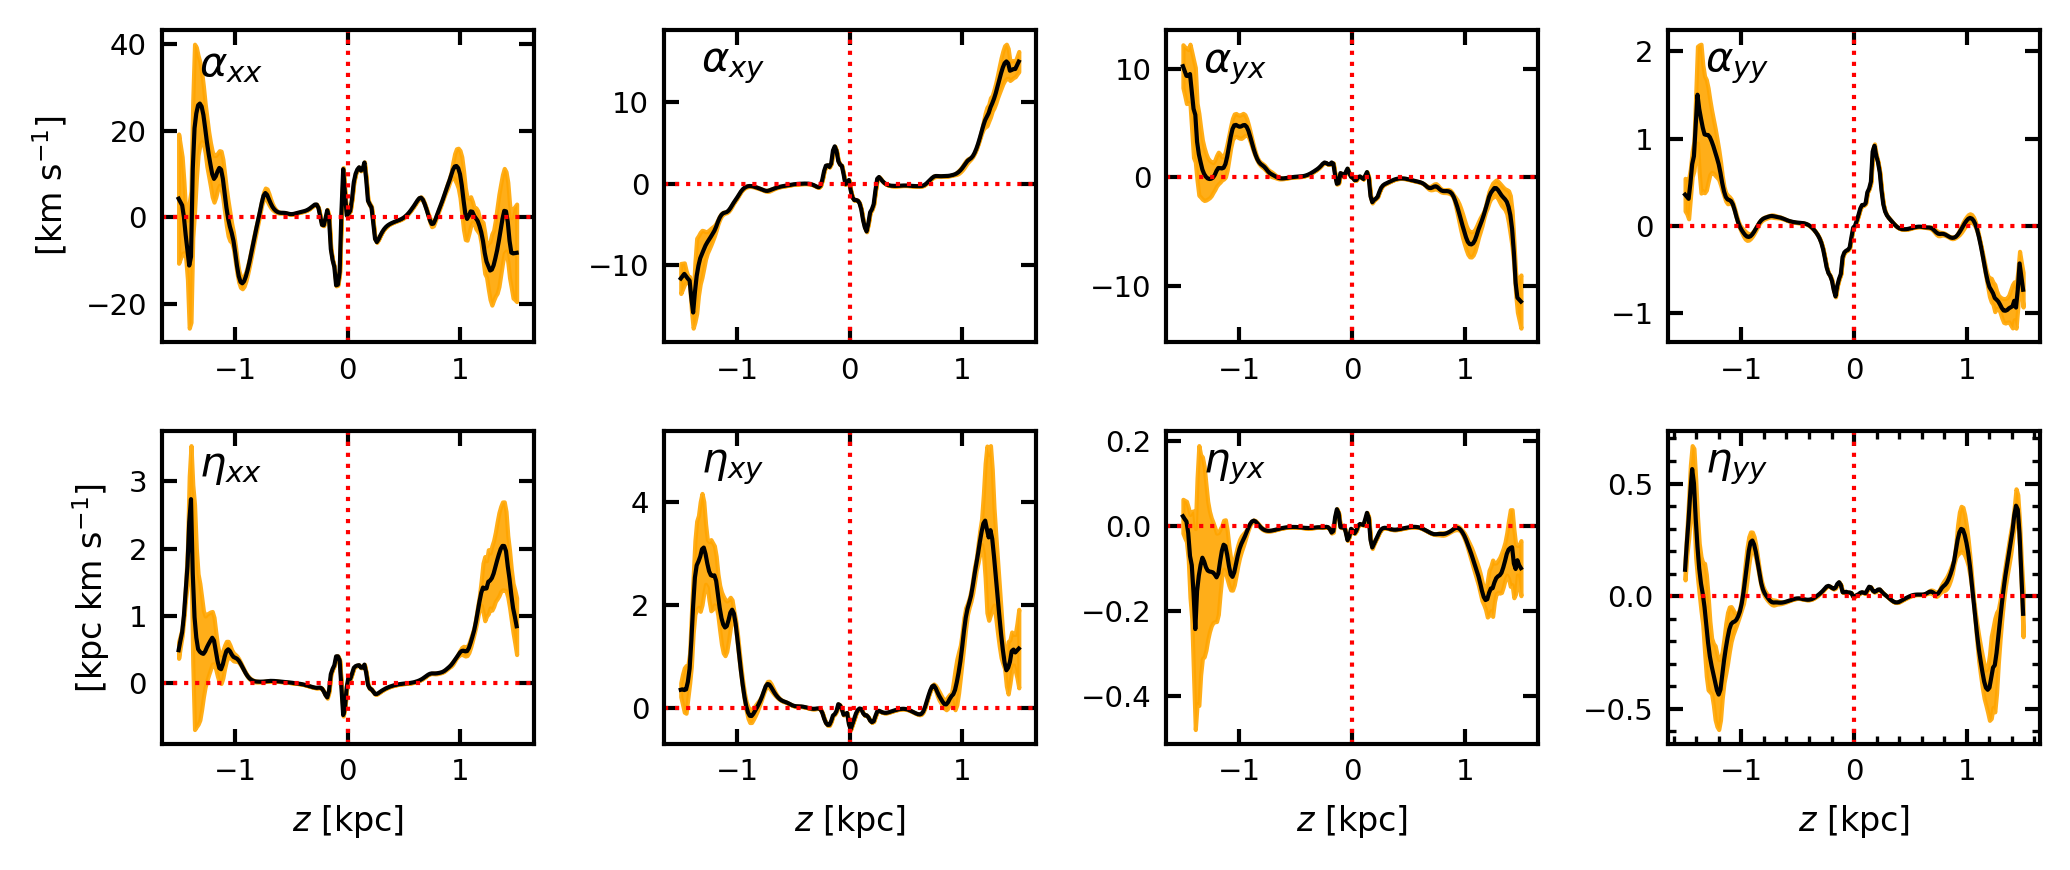
\includegraphics[width=\textwidth]{IROS_alpha_tensor.png}
   \caption{The {time-averaged component coefficients} of the turbulent
transport tensor introduced in Equation~\ref{EMF} for model \RSOBSD\ {during}
the nonlinear state at $1.0<t<1.5 \Gyr$. The yellow shading indicates one
standard deviation of {each component} based on bootstrap resampling of the
time series of {the EMF} $\mathcal{E}$.}
    \label{fig:IROS}
\end{figure*}
%--------------------------------------------------------------------------------

\subsection{Approximating the $\alpha$-effect}\label{sec:approx}

Some indication of EMF properties may be extracted from our imposed
$\alpha$-effect term. The action of the Coriolis force on the sheared,
vertically stratified disc will tend to inject helicity into the systemic
vertical flows of opposite signs on either side of the midplane. The dynamo
amplifies a magnetic field with opposing small-scale helicity, which will
quench the dynamo if it can not be removed \citep{Brandenburg_2005,SS21}. Under
the assumption of homogeneous isotropic turbulence $\vec{\upalpha}$ can be
reduced to a scalar
\begin{equation}
    \alpha = \alpha_k +\alpha_m\,.
    \label{alpha_scalar}
\end{equation}
The kinetic helicity contributes to the mean-field dynamo as
\begin{equation}
    \alpha_k \approx -\frac{1}{3}\tau \aver{\uu\cdot\vec{\omega}^\prime}\,,
    \label{alpha_k}
\end{equation}
where $\tau$ is the correlation time of the turbulence and $\vec{\omega}^\prime
= \nabla\times\uu$ is its vorticity \citep{Moffatt1978,1980mfmd_Krause_Radler}.
Due to the conservation of magnetic helicity, for the mean-field dynamo to
exist some small-scale helicity flux is required
\citep{PFL1976,Brandenburg_2005}. The magnetic helicity contributes to the
mean-field dynamo as
\begin{equation}
    \alpha_m \approx \frac{1}{3}\tau\left\langle\frac{(\nabla\times\BB)^\prime\cdot\BB^\prime}{\rho}\right\rangle\,.
    \label{alpha_m}
\end{equation}
These simplified expressions can be used to see how the Lorentz force acts
against the flow as the dynamo approaches saturation, where the opposite sign
of $\alpha_m$ can lead to $\alpha$-quenching. We approximate the proxy for
$\alpha = \alpha_k +\alpha_m$ in equations~\eqref{alpha_scalar} and
\eqref{alpha_k}. Since our simulations in Tab~\ref{tab:sims} include rotation,
the mean helicity of the flow $\langle
\vec{u}\cdot(\nabla\times\vec{u})\rangle$ can be driven by both the Lorentz and
Coriolis forces. The Coriolis force in a stratified, rotating system is the
cause of the conventional $\alpha$-effect with $\alpha_k>0$ for $z>0$ and
$\alpha_k(-z) = -\alpha_k(z)$ \citep[e.g., Section $7.1$ of][]{SS21}.

As with \citet{QSTGB23} at $t>0.75\Gyr$, at the onset of the nonlinearity,
magnetic buoyancy spreads the magnetic field out of the layer $\lvert z \rvert<
h_{\alpha}$, which is evident during the period $0.75\Gyr\leq t\leq 1.0\Gyr$.
While the asymmetry of $\alpha_k$ in $z$  is evident in Figure~\ref{fig:ak_am},
the sign of $\alpha_k$ is opposite to that of $\alpha$ produced by the Coriolis
force which is clearly shown for $t>1.2\Gyr$.  The imposed mean-field dynamo
action near the midplane, with $\alpha$ as given in Equation~\ref{eq:alpha} has
the conventional sign, with $\alpha>0$ at $z>0$.  The opposite sign of the
kinetic helicity implies that helical motion produced by imposed dynamo
saturates in the layer near the midplane \citep[e.g., Section $7.11$
of][]{SS21}. After some time there is the generation of helicity with the
conventional sign which is generated at altitudes of $\lvert z\rvert
>h_{\alpha}$.  This additional dynamo action, which we attribute to the
>Coriolis force, {would appear to be} responsible for the dramatic change in
>field parity.  The sign of $\alpha_m$ is shown in the lower panel of
>Figure~\ref{fig:ak_am} which, as expected, has the opposite sign to that of
>$\alpha_k$ and {has} a comparable magnitude.

%----------------------------------------------------------------------------
\subsection{IROS analysis of the EMF composition}\label{sec:emf}

To further verify and justify our interpretation of the results, we have
computed the components of the (pseudo-)tensor $\alpha_{ij}$ and tensor
$\beta_{ij}$ using the method of iterative removal of sources (IROS) introduced
by \citet{bendre2023iterative}. \fg{Using sliding time averages of the mean
magnetic field, \footnote{\fag{please confirm}}} the components of the electromotive force
$\mathcal{E}_i = \langle \vec{u}\times\vec{b} \rangle_i$ are approximated by
$\mathcal{E}_i = \alpha_{ij}\langle \vec{B_j}\rangle - \beta_{ij}(\nabla\times
\langle \vec{B} \rangle)_j$. Explicitly,
%--------------------------------------------------------------------------------
\begin{equation}\label{EMF}
\begin{pmatrix} \mathcal{E}_x\\ \mathcal{E}_y\end{pmatrix}
=\begin{pmatrix} \alpha_{xx} &\alpha_{xy}\\ \alpha_{yx} &\alpha_{yy} \end{pmatrix}
\begin{pmatrix} \mean{B}_x \\ \mean{B}_y \end{pmatrix}
-\begin{pmatrix} \beta_{xx} &\beta_{xy}\\ \beta_{yx} &\beta_{yy} \end{pmatrix}
\begin{pmatrix} (\nabla\times\mean{\vec{B}})_x \\ (\nabla\times\mean{\vec{B}})_y \end{pmatrix}
\end{equation}
%--------------------------------------------------------------------------------
are solved to determine the elements of the tensors $\alpha_{ij}$ and
$\beta_{ij}$, which are assumed to be independent of time. This assumption is
valid in either the early stages of the exponential growth of the magnetic
field or in the later, stationary state of the system. {These} calculations
{use} horizontal averaging{,} $\mean{\vec{B}}=\meanh{\vec{B}}$, as
displayed in Figure~\ref{fig:xy_averages}, such that the tensor elements are
functions of $z$ alone.  The horizontal average of the vertical component of
the magnetic field vanishes due to the horizontal periodic boundary conditions.
Hence, the analysis is applied only to the horizontal components of the
magnetic field.

When the mean gas velocity vanishes (as it does in this case) the equation for
the mean magnetic field has the form
%--------------------------------------------------------------------------------
\begin{equation}
    \deriv{\langle \vec{B} \rangle }{t} = \nabla \times (\mathcal{E}-\eta\nabla\times\langle\vec{B}\rangle)
\end{equation}
%--------------------------------------------------------------------------------
the diagonal elements of the $\alpha$-tensor represent the $\alpha$-effect with
$\alpha_k+\alpha_m \approx \dfrac{1}{2}(\alpha_{xx}+\alpha_{yy})$. If the flow
is isotropic in the ($x,y$)-plane $\alpha_{i,j}$ is antisymmetric ($\alpha_{yx}
= -\alpha_{xy}$) and the off-diagonal elements represent the transfer of the
mean magnetic field along the $z$-axis at the effective speed $U_z =
-\alpha_{xy}$ due to the increase in the turbulent magnetic diffusivity with
$\lvert z \rvert$ resulting mainly from the increase of the random flow speed
\citep[turbulent diamagnetism -- e.g., Section~7.9 of][]{SS21}. The diagonal
components of the tensor $\beta_{ij}$ represent the turbulent magnetic
diffusion.

Figure~\ref{fig:IROS} presents the resulting components of the tensors
$\alpha_{ij}$ and $\beta_{ij}$ for the nonlinear stage of the evolution. The
yellow shading spans one standard deviation of the variables obtained from five
estimates, each resulting from the sampling of every fifth iteration of 1500
with intervals of $1\Myr$ in the time series of $\mathcal{E}$ at each $z$.

The sum $\alpha_{xx}+\alpha_{yy}$ is significant in magnitude, antisymmetric
with respect to the midplane $z=0$ and mostly negative at $z>0$.  The
magnitudes of $\alpha_{xx}+ \alpha_{yy}$ are close to $\alpha_{k}+\alpha_{m}$
obtained using equations (\ref{alpha_k}) and (\ref{alpha_m}) during the
interval beyond $1\Myr$. The off-diagonal components of the $\alpha_{ij}$ are
quite close to the expected antisymmetry $\alpha_{yx}=-\alpha_{xy}$.  Near the
midplane these support an inward transfer of the mean magnetic field.  In
association with the increase of the turbulent magnetic diffusivity with
$\lvert z \rvert$, this will tend to oppose the buoyancy migration of the
magnetic field away from the midplane, thus leading to saturation of the MBI.
Te tensors $\alpha_{ij}$ and $\beta_{ij}$ fluctuate around the zero level
during the linear stage without any significant effect on its evolution.

%-----------------------------------------------------------------

\subsection{One-dimensional mean-field model}\label{sec:1D}

{To test our understanding of the role of the $\alpha^2\Omega$-dynamo and
MBI on the evolution of the mean field, and how this depends on the rates of
shear, rotation and scale height, we seek to replicate the 3D MHD solutions
above using} a nonlinear one-dimensional {(1D)} model{. We model} the
mean-field dynamo with advection due to magnetic buoyancy and demonstrate that
it not only admits parity switches seen in the {3D} models presented but
also reproduces quantitatively the resultant field.

Improving upon the model shown in \citet{QSTGB23} we include the effects of
differential rotation and now account for the complex structure of the kinetic
helicity generated in the nonlinear phase by magnetic buoyancy and differential
rotation.  {We model each component of the magnetic field as}
%------------------------------------------------------------------------------
\begin{align}
\deriv{B_x}{t} &= -\deriv{}{z}(\alpha B_y)+\beta\dfrac{\partial^2 B_x}{\partial z^2} - \deriv{}{z} (B_yU_z - B_zU_y)\label{1DBx}, \\
\deriv{B_y}{t} &= \deriv{}{z}(\alpha B_x)+\beta\dfrac{\partial^2 B_y}{\partial z^2} - \deriv{}{z} (B_xU_z - B_zU_x) + S_0B_x\label{1DBy} \\
\nonumber
\text{and}& \\
\deriv{B_z}{t} &= \alpha B_y + \beta\dfrac{\partial^2B_z}{\partial z^2} - \deriv{}{z}(U_xB_y-U_yB_x)\label{1DBz},
\end{align}
%------------------------------------------------------------------------------
where $S_0=-25 \kms\kpc^{-1}$\footnote{\fag{Why do we restrict this to 25?
Which 3D model are we therefore comparing? In figure 8 we contrast with model
\RSOBSD, which would indicate $S_0=-18 \kms\kpc^{-1}$.}} is the shear rate and
we assume that all variables only depend on $t$ and $z$ (the infinite slab
approximation).  \fg{Here $\alpha$ is as specified by Equation~\eqref{eq:alpha}
and $\beta$?\footnote{\fag{How does $\beta$ relate to $\eta$ or other
parameters in the 3D model?}} The initial magnetic field has a strength of
$10^{-3} \mu G$.}

%------------------------------------------------------------------------------
\begin{figure}
    \centering
    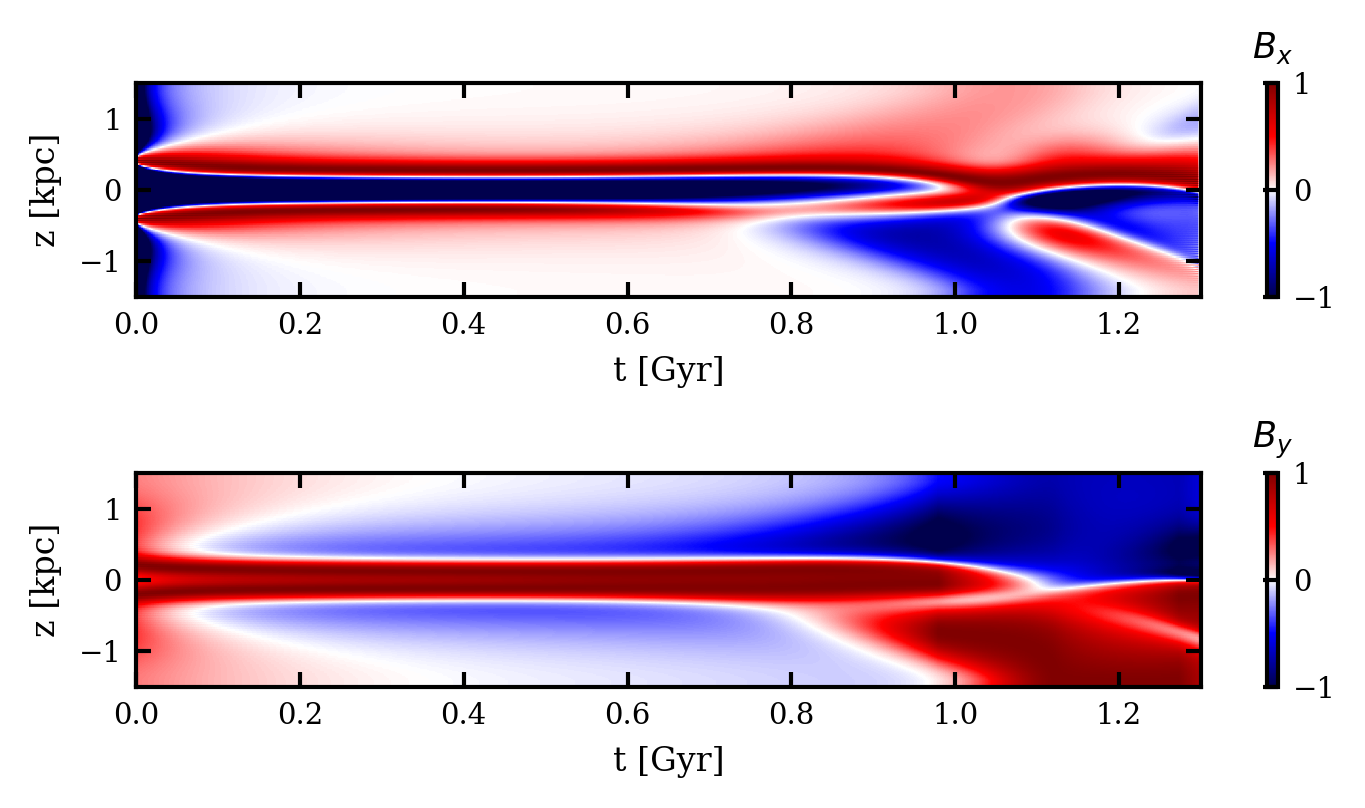
\includegraphics[width=0.5\textwidth]{1D_xy_aver.png}
    \caption{The evolution magnetic field components $\langle \widehat{B}_x\rangle_{xy}$ (upper panel) and $\langle \widehat{B}_y\rangle_{xy}$ (lower panel) for the 1D model using parameters which match model {\RSOBSD}. The magnetic field components are normalized to their maximum values at each time.}
    \label{fig:1D_xy}
\end{figure}
%------------------------------------------------------------------------------

{We} omit brackets denoting the averaging to simplify notation in this
section{, including} the velocities $U_x$, $U_y$ and $U_z$ {averaged} at
an intermediate scale between the turbulen{ce} and {the size of the disc}.
We additionally solve {their} Navier-Stokes equations
\begin{align}
    \deriv{U_x}{t} &= B_z\deriv{B_x}{z} + 2U_y\Omega + \nu \frac{\partial^2 U_x}{\partial z^2}\label{1DUx},\\
    \deriv{U_y}{t} &= B_z\deriv{B_y}{z} + 2U_x\Omega + \nu \frac{\partial^2 U_x}{\partial z^2} - SU_x\label{1DUy},\\
    \nonumber
    \text{and}& \\
    \deriv{U_z}{t} &= - B_y\deriv{B_y}{z} - B_x\deriv{B_x}{z} + \nu \frac{\partial^2 U_x}{\partial z^2} - \frac{1}{8\pi\rho}\deriv{B^2}{z} +\frac{\rho^\prime}{\rho_0}g,\label{1DUz}
\end{align}
%------------------------------------------------------------------------------
where $g$ is the vertical acceleration due to gravity and the second
term\footnote{\fag{which term of which equation? Why do all equation depend on
the vertical gradient only of $U_x$?}} on the right-hand side is the Archimedes
force resulting from magnetic buoyancy.  \fg{The initial velocity is at rest.}\footnote{\fag{Is this correct?}}

  We neglect the time variation of the gas density, adopting $\rho =
\rho_0(z)$\footnote{\fag{Using what profile?}} at all times but, in the spirit
of the Boussinesq approximation, include density variation $\rho^\prime$ in the
Archimedes force.  Consider{ing} a region of density $\rho = \rho_0
+\rho^\prime$ containing a magnetic field of a strength $B+b$ surrounded by the
gas of the density $\rho_0$ with magnetic field $B$ (here $B$ is the mean field
strength and b\footnote{\fag{Is $b$ fixed and how? Does $\rho^\prime$ evolve,
presumably as $B$ evolves?}} is its local perturbation) {the} pressure
balance in an isothermal gas then leads to
%------------------------------------------------------------------------------
\begin{equation}
    \rho^\prime = -\dfrac{2Bb+b^2}{8\pi c_s^2}\,.
\end{equation}

Crucially, the averaging condition used here must exclude the horizontal
average, {which is applied in Section~\ref{sec:emf} and
Figures~\ref{fig:xy_averages}--\ref{fig:IROS},} since the field average in the
horizontal (x,y)-plane is a function of $z$ alone. Combined with
$\nabla\cdot\mathbf{B} = 0 \Rightarrow \partial\langle B_z\rangle/\partial
z=0$.  Although horizontal averaging satisfies the Reynolds rules, its
restrictions limit the admissible structure of the magnetic field, without any
physical or mathematical justification.  If such an averaging method were used,
then there could be no evolution equation for $B_z$.  This indicates that
important information is lost when considering a horizontally averaged field
and that the horizontal spatial structure of all components of the magnetic
field should be accounted for as they may produce non-trivial effects.

Equations \eqref{1DBx}{--}\eqref{1DUz} are solved numerically in
$-z_0<z<z_0$ with $z_0=1.5\kpc$. Initially,\footnote{\fag{Is the velocity not
initially 0?}} $B_x$, $B_y$ and $B_z$ are symmetric about $z=0$ (a quadrupolar
magnetic structure and known to dominate within a thin layer - e.g., Section
11.3.1 of \citealt{SS21}).
% %------------------------------------------------------------------------------
% \begin{equation}
%     \deriv{B_x}{z} = \deriv{B_y}{z} = \deriv{B_z}{z} = U_z = 0
% \end{equation}
%------------------------------------------------------------------------------
At $z=z_0$ we apply an impenetrable boundary condition for $U_z$, and vacuum boundary conditions for the magnetic field
%------------------------------------------------------------------------------
\begin{equation}
    U_z = B_x = B_y = B_z = 0{.}
\end{equation}
%------------------------------------------------------------------------------
We justify this {given} the turbulent magnetic diffusivity increases with
$\lvert z \rvert$ (see Section 11.3 of \citealt{SS21}, for details). Larger
vertical sizes were {tested} to confirm the domain was large enough to
prevent any spurious boundary effects over the simulation period.

Figure~\ref{fig:1D_xy} shows the evolution of the horizontally averaged
magnetic field components and the switch in field parties. The {1D} model in
Figure~\ref{fig:1D_xy} reproduces quantitatively
Figure~\ref{fig:xy_averages}\footnote{\fag{What does this mean? Both plots are
normalised to 1, so only display topology evolution. Do you mean Fig 4?}} and
on a similar timescale to the full {3D} model, the main point being the
switch in parity due to the inclusion of the differential rotation. We do not
attempt to achieve a precise match between the {3D} and {1D} results
being content with the fact that the {1D} model justifies further our
conclusion that the change in field parity is a nonlinear phenomena that rely
on the interaction of the mean-field dynamo and the rotational shear.

{Adjusting the parameters in the 1D model and varying which terms are
included enables us to verify that all terms are essential to replicate the 3D
MHD solutions.  Changing the rate of shear $S$\footnote{\fag{does what with a critcal
rate of shear? For $h_\alpha, \alpha_0$, $\nu$ and $\beta$, one at a time
and specify what changes in the solution at what are critical parameter values
that alter the qualitative solution; growth rates, parity switches, period of
reversals?. Replace these specific quantifiable statements for the paragraph
below}} \yq{The key parameters which alter the solution are the dynamo scale height
$h_\alpha, \alpha_0$, the shear rate $s$ and the diffusion coefficients $\nu$
and $\beta$. Increasing the scale height of the dynamo has the effect of
increasing the scale height of the magnetic field but causes no discernible
change in the parity of the field when the dynamo number is kept constant
(changing $\alpha_0$ to keep the same dynamo number). Having larger values of
diffusion causes the magnetic field to decay quicker and means that larger
values of $\alpha_0$ are needed for the magnetic field to grow.}

\section{Summary and implications}\label{sec:Summary}

The nonlinear interaction of the mean-field dynamo and magnetic buoyancy leads
to profound changes in the evolution of the large-scale magnetic field whose
properties are beyond what may be found in a study of the early stages of
magnetic field amplification (when the Lorentz force is still negligible).
Magnetic buoyancy spreads the magnetic field into the corona of the galaxy.
{The} large-scale field{,} under the effects of differential
rotation{,} generates a kinetic helicity with the opposite sign to the
helicity of the imposed $\alpha$-effect from which the large-scale field was
generated.

When the buoyant magnetic field is not helical (e.g. unidirectional) and there
is no rotation, magnetic buoyancy will only redistribute the large-scale
magnetic field to larger altitudes reducing very strongly its pressure gradient
and leaving the support of the gas layer against the gravity to
\fg{only}\footnote{\fag{is this what is meant?}} the thermal pressure gradient
and contributions from turbulence and random magnetic fields if present
\citep{DT2022b}.

The inclusion of the rotation changes the picture because the gas flows that
accompany magnetic buoyancy become helical driving a mean-field dynamo that in
\citet{DT2022a} is able to overwhelm an imposed magnetic field leading to a
reversal, which indicates the potential of magnetic oscillations. In our case
the resultant complex structure of the kinetic helicity{,} which occurs due
to the combined Lorentz and Coriolis forces{,} is responsible for the change
in magnetic field parity seen in the nonlinear stages of the system.
\citet{DT2022a} examine the effects of rotation and shear alongside an imposed
magnetic field, rather than dynamo generated, but do not discuss the field
parity of the stationary state.

{We verify this conclusion using a simple 1D model. The solution to the
equations of the $1$D model used in \citet{QSTGB23} in Section~\ref{sec:1D}
without any terms expressing the differential rotaion of the system does not
permit solutions to the nonlinear state with switches to the parity.  In our
solutions to the modified equations in Section~\ref{sec:1D} we are able to
replicate this change in parity, if and only if the effects of the rotation and
shear are included.}

The consequences of the interaction{s between} the
{$\alpha^2\Omega$-}dynamo and magnetic buoyancy {instability} depend on
the {intensity of each process as well as the} relative intensities of the
two processes. {This will} vary {both across differing locations} within
a galaxy and between {differing} galaxies.  The {$\alpha^2\Omega$-}dynamo
efficiency {increases with} the scale height of the gas and {with higher
rates of galactic shear}.  {This will generate preferentially even-parity,
typically quadrupolar} magnetic fields in a thin disc.  This preference for
even solutions is explained by the fact that the shortest vertical scale of a
quadrupolar horizontal field is twice as large as that of a dipolar magnetic
structure. Magnetic diffusion would then act four times faster on dipolar than
quadrupolar fields, making the maintenance of a dipolar field difficult.
{The magnetic buoyancy instability efficiency, however, is enhanced as the
scale height reduces of the horizontal magnetic field and correspondingly of
the gas density. MBI effects would therefore be most apparent where the disc is
particularly thin and also supports a strong planar magnetic field.} 

Even parity fields in galactic discs are a firm prediction of dynamo
theory{.  However,} it is possible, and the results shown in this work seem
to support, that a dipolar field within a kiloparsec of the disc axis {can
support dipolar modes where} the dynamo number is sufficiently large enough.
{Here, where the scale height tends to be narrower, magnetic buoyancy
instability can also sustain dipolar modes.\footnote{Add some further
quantifiable statements once the table has been updated.}}

The rotation speed reduces with distance from the disc of the spiral galaxy,
this has been firmly established by observation of neutral and ionized
hydrogen. \citet{LHB2008} find $\partial V_{\phi}\partial/\lvert z\rvert =
-(22\pm 6)\kms$ within $\lvert z\rvert = 100\p$ of the Galactic midplane near
the sun. Since the $D\sim \Omega^2$ this will dramatically weaken the
mean-field dynamo at larger altitudes and because this switch in dipolar parity
requires dynamo action at larger altitudes. If vertical rotation speed
variation were accounted for, the switch to dipolar parity would require a
stronger mean-field dynamo.


Our simulations are performed in a relatively large but still limited, limited
part of a gas layer ($2 \times 2\kpc$ horizontally) using Cartesian
coordinates. The computational domain is large enough to accommodate the most
rapidly growing mode of the MBI and, the results likely would not be much
different in cylindrical coordinates where the unstable magnetic field is not
unidirectional. Therefore, it is reasonable to expect that our main conclusions
apply to galactic and \fg{accretion}\footnote{\fag{Is this a typo? recreation}}
discs {in general,} at least at some distance from the disc axis where the
curvature may not be as strong.

\section*{Acknowledgements}
The authors benefited from valuable discussions at the Nordita workshop
`Towards a Comprehensive Model of the Galactic Magnetic Field' at Nordita
(Stockholm) in 2023, supported by NordForsk and Royal Astronomical Society.
FAG acknowledges support of the Finnish Ministry of Education and Culture
Global Programme USA Pilot 9758121 and the Swedish Research Council
(Vetenskapsrådet) grant no. 2022– 03767.

%%%%%%%%%%%%%%%%%%%%%%%%%%%%%%%%%%%%%%%%%%%%%%%%%%
\section*{Data Availability}

The raw data for this work were obtained from numerical simulations using the open source PENCIL-CODE available at \url{https://github.com/pencil-code/pencil-code.git}. The derived data used for the analysis given in the paper is available on reasonable request from the corresponding author.




%%%%%%%%%%%%%%%%%%%% REFERENCES %%%%%%%%%%%%%%%%%%

% The best way to enter references is to use BibTeX:

\bibliographystyle{mnras}
\bibliography{refs} % if your bibtex file is called example.bib


% Alternatively you could enter them by hand, like this:
% This method is tedious and prone to error if you have lots of references
%\begin{thebibliography}{99}
%\bibitem[\protect\citeauthoryear{Author}{2012}]{Author2012}
%Author A.~N., 2013, Journal of Improbable Astronomy, 1, 1
%\bibitem[\protect\citeauthoryear{Others}{2013}]{Others2013}
%Others S., 2012, Journal of Interesting Stuff, 17, 198
%\end{thebibliography}

%%%%%%%%%%%%%%%%% APPENDICES %%%%%%%%%%%%%%%%%%%%%

% \appendix

% \section{Some extra material}

% If you want to present additional material which would interrupt the flow of the main paper,
% it can be placed in an Appendix which appears after the list of references.

%%%%%%%%%%%%%%%%%%%%%%%%%%%%%%%%%%%%%%%%%%%%%%%%%%


% Don't change these lines
\bsp	% typesetting comment
\label{lastpage}
\end{document}

% End of mnras_template.tex
